\section{Постановка задачи и основные соотношения}
%Будем рассматривать рассеяние плоской электромагнитной волны на рассеивателях в различных диапазонах частот для шариков, состоящих из серебра, меди и золота. Представим шарики ввиде сфер и рассмотрим три случая, для одиночной сферы Рис.\ref{fig:1st_scatterer}, для 5 сфер Рис.\ref{fig:2nd_scatterer} и для 17 сфер Рис.\ref{fig:3td_scatterer}. Однако пред этим, найдем рассеянние на цилиндре численным и точным методом решения, чтобы убедиться в правильности получаемых данных. \\
Будем рассматривать рассеяние плоской монохроматической электромагнитной волны на рассеивателях различной геометрии в широком диапазоне частот. Поле такой электромагнитной волны описывается следующим образом
\begin{align}
	&\vec{E}= \vec{x}_0{E}_{0} \exp (i\omega t - i k_0z)\\
	&\vec{H}= \vec{y}_0{E}_{0} \exp (i\omega t - i k_0z)
\end{align}
В качестве рассеивателей будет рассматриваться несколько самоподобных (фрактальных) объектов увеличивающейся сложности. Так, на <<нулевой>> итерации рассеиватель --- это просто однородный шар (см. Рис. \ref{fig:1st_scatterer}); на второй --- пять шаров (см. Рис.\ref{fig:2nd_scatterer}), наибольший из которых совпадает с шаром на предыдущей итерации, а 4 малых шара имеют радиусы в 2 раза меньше радиуса большой сферы; на третьей итерации --- 17 шаров (см. Рис. \ref{fig:3td_scatterer}), самые малые шары имеют радиусы в 2 раза меньше, чем радиусы малых шаров на предыдущей итерации. Все центры шаров располагаются в плоскости $xOy$. Материалы всех элементов, составляющих рассеиватели считаем одинаковыми. В качестве вещества, заполняющего шары, будем рассматривать серебро, медь и золото. Ввиду хорошей проводимости этих веществ на низких частотах элементы рассеивателей могут быть заменены тонкостенными сферами, из-за присутствия скин--эффекта в этих диапазонах длин волн.
\newpage
\begin{figure}[h!]
	\centering
	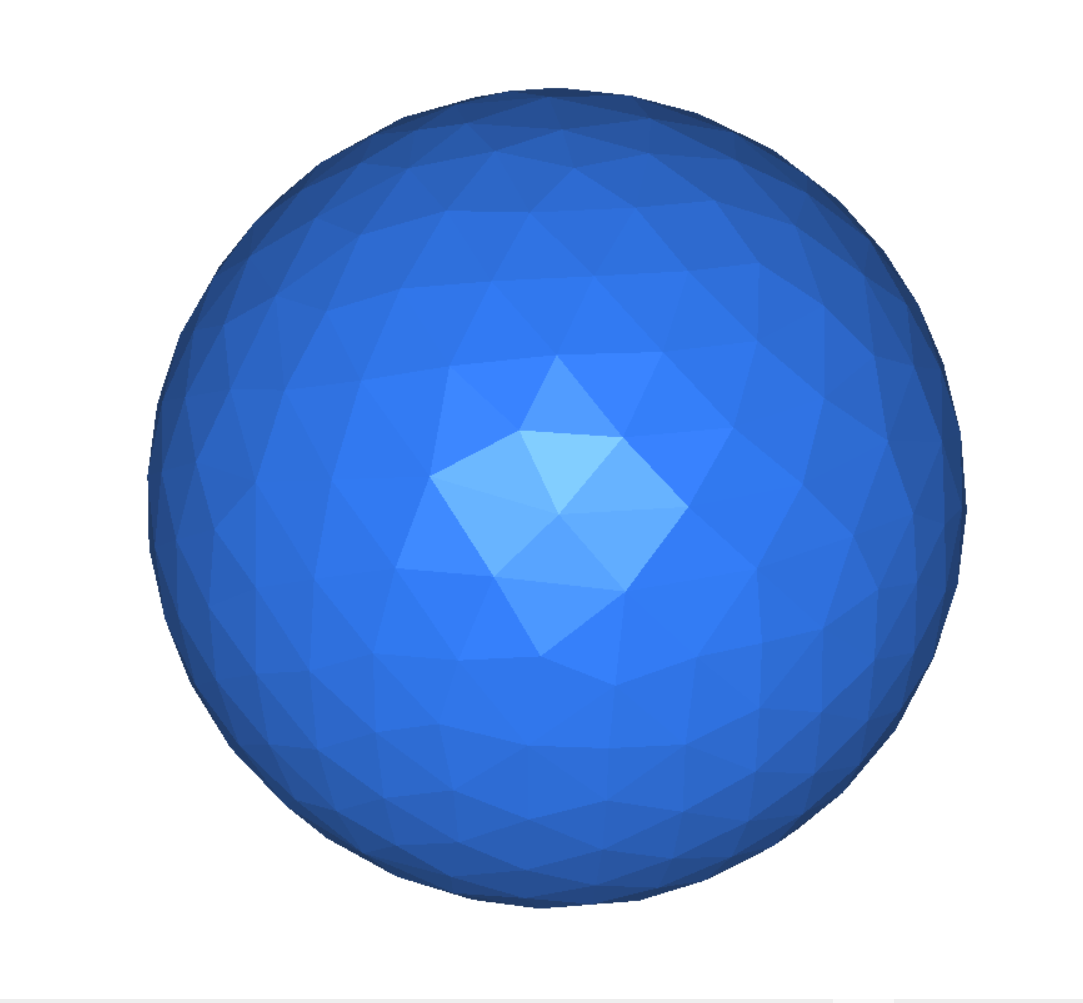
\includegraphics[width=0.4\linewidth]{1st_scatterer}
	\caption{Единичная сфера}
	\label{fig:1st_scatterer}
\end{figure}
\begin{figure}[h!]
	\centering
	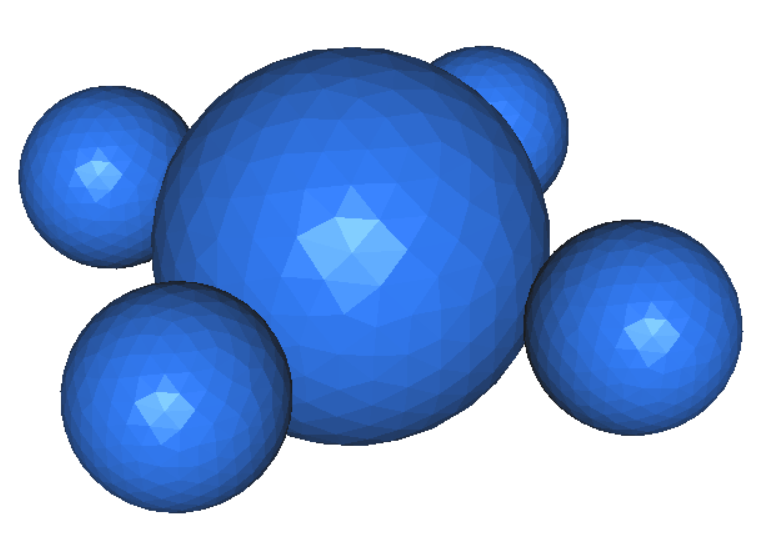
\includegraphics[width=0.5\linewidth]{2nd_scatterer}
	\caption{Первая итерация - 5 сфер}
	\label{fig:2nd_scatterer}
\end{figure}
\begin{figure}[h!]
	\centering
	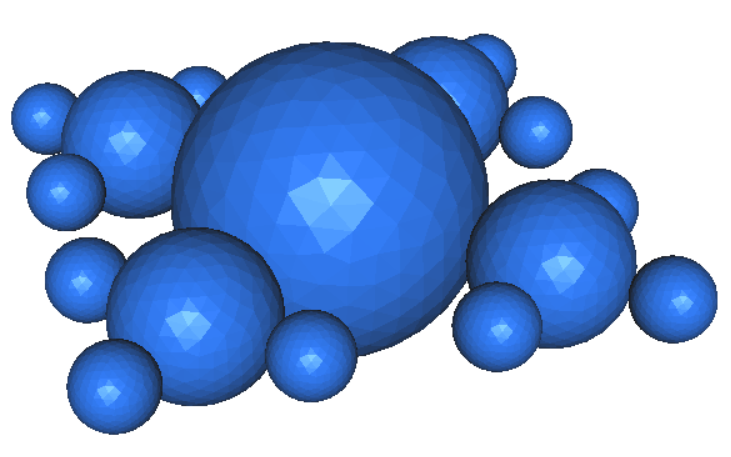
\includegraphics[width=0.5\linewidth]{3td_scatterer}
	\caption{Вторая итерация - 17 сфер}
	\label{fig:3td_scatterer}
\end{figure} 
\section{Описание метода решения задачи}
Запишем уравнения Максвелла:
\begin{align}
 {\rm rot}\vec{E} &= -\dfrac{1}{c}\dfrac{\partial \vec{B}}{\partial t} \\
 \rm rot\vec{H} &=\dfrac{4\pi}{c}\vec{j} + \dfrac{1}{c}\dfrac{\partial \vec{D}}{\partial t} \\
 \rm div\vec{D} &= 4\pi \rho \\
 \rm div\vec{B} &= 0 
\end{align}
При этом не забыв про материальные уравнения, описывающие характеристики среды, в которой распространяется электромагнитная волна:
\begin{align}
	   \vec{D} &= \varepsilon \vec{E}\\
	   \vec{B} &= \mu \vec{H} \\
	   \vec{j} &= \gamma \vec{E}
\end{align}
Здесь $\varepsilon$ --- диэлектрическая проницаемость среды, $\mu$ --- магнитная проницаемость среды, $\gamma$ --- проводимость среды. Будем решать задачу дифракции плоской волны на рассматриваемых рассеивателя с использованием метода конечных элементов. Для этого наш объект заключим в сферическую расчётную область, в которой будем находить рассеиваемые волны. Сразу определим, что наибольший размер рассматриваемого рассеивающего объекта по одному измерению будет меньше длины волн, а радиус $R$ расчётной сферической области будет в 4 раза больше длины волны (Рис. \ref{fig:ces1}). Так же стоит отметить, что на протяжении всей работы будет использоваться гармоническая зависимость $ e^{i \omega t} $, где $ i = \sqrt{-1} $. 

%Далее найдем сечение рассеяния $ \sigma_s $ и сечение поглощения $ \sigma_a $, которое будет находиться на удалении $ \lambda = 3 $, с помощью действительной $ \varepsilon' $ и мнимой $ \varepsilon'' $ части диэлектрической проницаемости на основе коэффициентов преломления $ n' $ и $ n'' $. Сделаем тоже самое для всех трех случаев.  Для удобства поиска решения расчеты будем производить в декартовой системе координат.
\begin{figure}[h!]
	\centering
	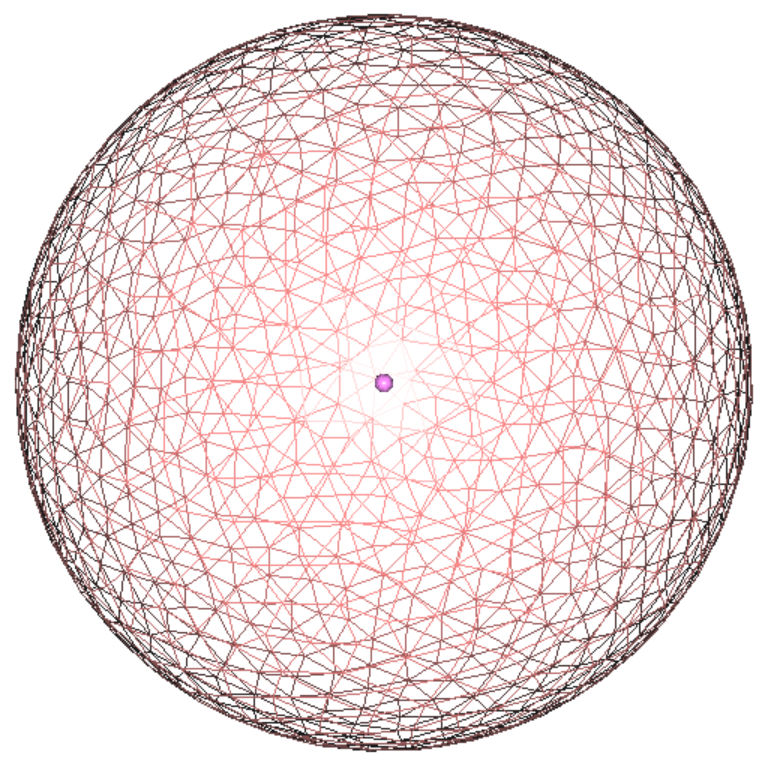
\includegraphics[width=0.4\linewidth]{ces1}
	\caption{}
	\label{fig:ces1}
\end{figure}


Найдём уравнения для сформулированной задачи в <<слабой>> форме, которые пригодны для использования в методе конечных элементов. Для этого, прежде всего, обратимся к рис.\ref {fig:tes2}, на котором представлены различные рассеивающие объекты.
\begin{figure}[h]
	\centering
	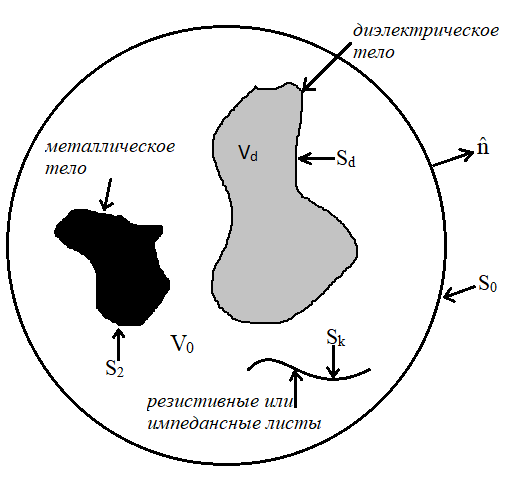
\includegraphics[width=0.6\linewidth]{tes2}
	\caption{}
	\label{fig:tes2}
\end{figure}
Вычислительная область ($ V_{0} $) ограничена поверхностью ($ S_{0} $) и может содержать различные рассеивающие объекты, такие как неоднородные диэлектрики ($ V_{d} $), металлические тела ($ S_{2} $) и резистивные или импедансные листы ($ S_{k} $). Метод конечных элементов позволяет легко моделировать рассеиватели произвольной формы и неоднородные области, не предъявляя жестких требований к их форме, размеру и составу. Ввиду того, что наш интерес ограничен рассеянием, плотности электрического и магнитного токов будут равны нулю.
С учетом граничных условий на рассеивателях, следует рассмотреть его средневзвешенное значение, дающее так называемую слабую форму векторного волнового уравнения. Домножая на векторную функцию $ \vec{\cal{E}} $ волновое уравнение для поля $\vec{E}$, полученное из уравнений Максвелла, приходим к выражению:
\begin{equation}\label{a1}
	\iiint\limits_{V_{0}}^{} \left\{\left[ \nabla \times \left[ \dfrac{1}{\mu_{r}}\nabla \times \vec{E}\right]\right]\cdot \vec{\cal{E}} - k_{0}^{2} \varepsilon_{r}\vec{E} \cdot \vec{\cal{E}} \right\}d\upsilon = 0
\end{equation}
Здесь $\mu_r$ и $\varepsilon_r$ --- функции, задающие распределение диамагнитной и диэлектрической проницаемости в рассматриваемой области. Однако уравнение (\ref{a1}) должно выполняться для каждого из малых объемов, а не в каждой точке $ V_{0} $. Используя первую векторную формулу Грина, с учётом уравнений Максвелла, можем переписать формулу (\ref{a1}): \\
\begin{equation}
\iiint\limits_{V_{0}}^{} \left[ \dfrac{1}{\mu_{r}}[\nabla \times \vec{E}] \cdot [\nabla \times \vec{\cal{E}}] - k_{0}^{2} \varepsilon_{r}\vec{E} \cdot \vec{\cal{E}} \right]d\upsilon - i k_{0} \oiint\limits_{S_0} [\hat{n} \times \vec{H}] \cdot \vec{\cal{E}}ds = 0,
\end{equation}
где $ \vec{H} $ - полное магнитное поле, удовлетворяющее уравнению Максвелла, $ \vec{E} $ - полная напряженность электрического поля, $ k_{0} $ - волновое число в свободном пространстве. Мы можем решить полученное уравнение численно для $ \vec{E} $, дискретизировав объем $ V_{0} $ и представив $ \vec{E} $ подходящим, скажем, линейным разложением внутри каждого из подобъемов $V_{e}$. Также необходимо обеспечить соблюдение всех необходимых граничных условий в пределах $V_{0}$ и на $S_{0}$, что подразумевает исключение $\vec{H}$, связав его с $\vec{E}$.

Учитывая, что наш интерес заключается в получении рассеянного поля телом, освещённым плоской волной, то $S_{0}$ служит только в качестве искусственной поверхности для ограничения бесконечной вычислительной области. В самом деле, если $S_{0}$ находится далеко от рассеивателя, мы можем тогда вызвать условие излучения Зоммерфельда и с учётом уравнений Максвелла получим соотношение:
\begin{equation}\label{a2}
	\left[\hat{r} \times \vec{H}^{scat}\right] = \left[\hat{r} \times \left[\hat{r} \times \vec{E}^{scat}\right]\right]
\end{equation}
		связав $ \vec{H} $ и $ \vec{E} $, где $ \hat{r} $ - нормаль к сферической поверхности $ S_{0} $ и
\begin{equation}
	\vec{H}^{scat} = \vec{H} - \vec{H}^{inc},\quad \vec{E}^{scat} = \vec{E} - \vec{E}^{inc}
\end{equation}
обозначают рассеянные поля, возбуждаемые плоской волной, описываемой полями ($ \vec{E}^{inc} $, $ \vec{H}^{inc} $).
Очевидно, что требование, чтобы $ S_{0} $ располагалась далеко от рассеивателя, значительно увеличивает вычислительный объем, что приводит к непрактично большим системам при дискретизации уравнения. Это побудило к использованию поглощающих граничных условий более высокого порядка, которые можно ставить на поверхности, находящейся в ближней зоне рассеивателя, без существенного снижения точности решения. Их целью является устранение обратных отражений от $ S_{0} $. Они обеспечивают приблизительную связь между $\vec{E}$ и $\vec{H}$ на поверхности $ S_{0} $, которую мы получаем, предполагая, что разложение поля пропорционально в степени $r$ (где $r$ --- расстояние от центра поверхности $S_{0}$). Если поглощающие граничные условия зануляют первые $(2m + 1)$ членов разложения по $r$, то их называют поглощающими граничными условия $m$-го порядка.
Поглощающие граничные условия нулевого порядка являются условием излучения Зоммерфельда, приведенным в формуле (\ref{a2}), а их представление второго порядка имеет вид:
\begin{equation}\label{a3}
	-i k_{0}\hat{n} \times \vec{H}^{scat} = i k_{0}\vec{E}_{t}^{scat} + \beta \nabla \times [\hat{n}(\nabla \times \vec{E}^{scat})_{n}] + \beta\nabla_{t} (\nabla \cdot \vec{E}_{t}^{scat}).
\end{equation}
В этом уравнении $ \hat{n} $ обозначает внешнюю нормаль к $S_{0}$, $\beta = 1/{2[i k_{0} + (1/r)]}$, а нижние индексы $t$ и $n$ обозначают тангенциальную и нормальную компоненты для $ S_{0} $ соответственно. 
Поглощающие граничные условия (уравнение (\ref{a3})) были получены для сферической поверхности $ S_{0} $, однако, они хорошо работают, когда $ S_{0} $ является кусочно-плоской, чтобы она лучше соответствовала поверхности рассеивателя.
В этом случае $ \beta $ сводится к $ \beta = 1/(2 i k_{0}) $. Точно так же мы можем обобщить уравнение (\ref{a2}) для кусочно-плоских поверхностей, положив $ \hat{r} \rightarrow \hat{n} $. Отметим, что, поскольку данные поглощающие граничные условия связывают рассеянные поля, лучше всего переписать формулу (\ref{a1}) в терминах рассеянных полей. Делая так, мы получаем:
\begin{align}\label{a4}
	&\iiint\limits_{V_{0}}^{} \left[ \dfrac{1}{\mu_{r}}(\nabla \times \vec{E}^{scat}) \cdot (\nabla \times \vec{\cal{E}}) - k_{0}^{2} \varepsilon_{r}\vec{E}^{scat} \cdot \vec{\cal{E}} \right]d\upsilon + 
	\iint\limits_{S_{0}}^{}  P(\vec{E}^{scat}) \cdot \vec{\cal{E}}ds +\notag\\
	&+ 
	\iiint\limits_{V_{d}}^{} \left[ \dfrac{1}{\mu_{r}}(\nabla \times \vec{E}^{inc}) \cdot (\nabla \times \vec{\cal{E}}) - k_{0}^{2} \varepsilon_{r}\vec{E}^{inc} \cdot \vec{\cal{E}} \right]d\upsilon +\notag\\
	&+ i k_{0}\iint\limits_{S_{d}}^{} \dfrac{1}{\mu_{r}}(\hat{n} \times \vec{H}^{inc}) \cdot \vec{\cal{E}}ds = 0,
\end{align}
в котором $P(\vec{E^{scat}})$ равно представлению в правой части уравнения (\ref{a2}), $ V_{d} $ - это объем, занимаемый диэлектриками, а $ S_{d} $ - это поверхности границ раздела сред. Мы вывели последние два интеграла в формуле (\ref{a4}) снова вызвав первое векторное тождество Грина и отметим, что ${ \vec E}^{inc} $ удовлетворяет волновому уравнению вектора свободного пространства. Очевидно, что (\ref{a4}) относится только к неизвестным $ {\vec E}^{scat}$, и мы можем приступить к его решению.



Далее найдем сечение поглощения $ \sigma_a $ и аналог сечения рассеяния $ \sigma_s $, которое будет находиться на расстоянии трёх длины волны от центра рассеивателя. Для этого будут использованы действительная $ \varepsilon' $ и мнимая $ \varepsilon'' $ части диэлектрической проницаемости, находимые на основе экспериментальных данных о коэффициентах преломления $ n' $ и $ n'' $.

На Рис.~\ref{fig:3td_scattererAndOuterSpheres} можно увидеть случай с 17 сферами, где в центре находится сам объект, окруженный сечением рассеяния, заключенный в сферическую область.\\
\begin{figure}[h!]
	\centering
	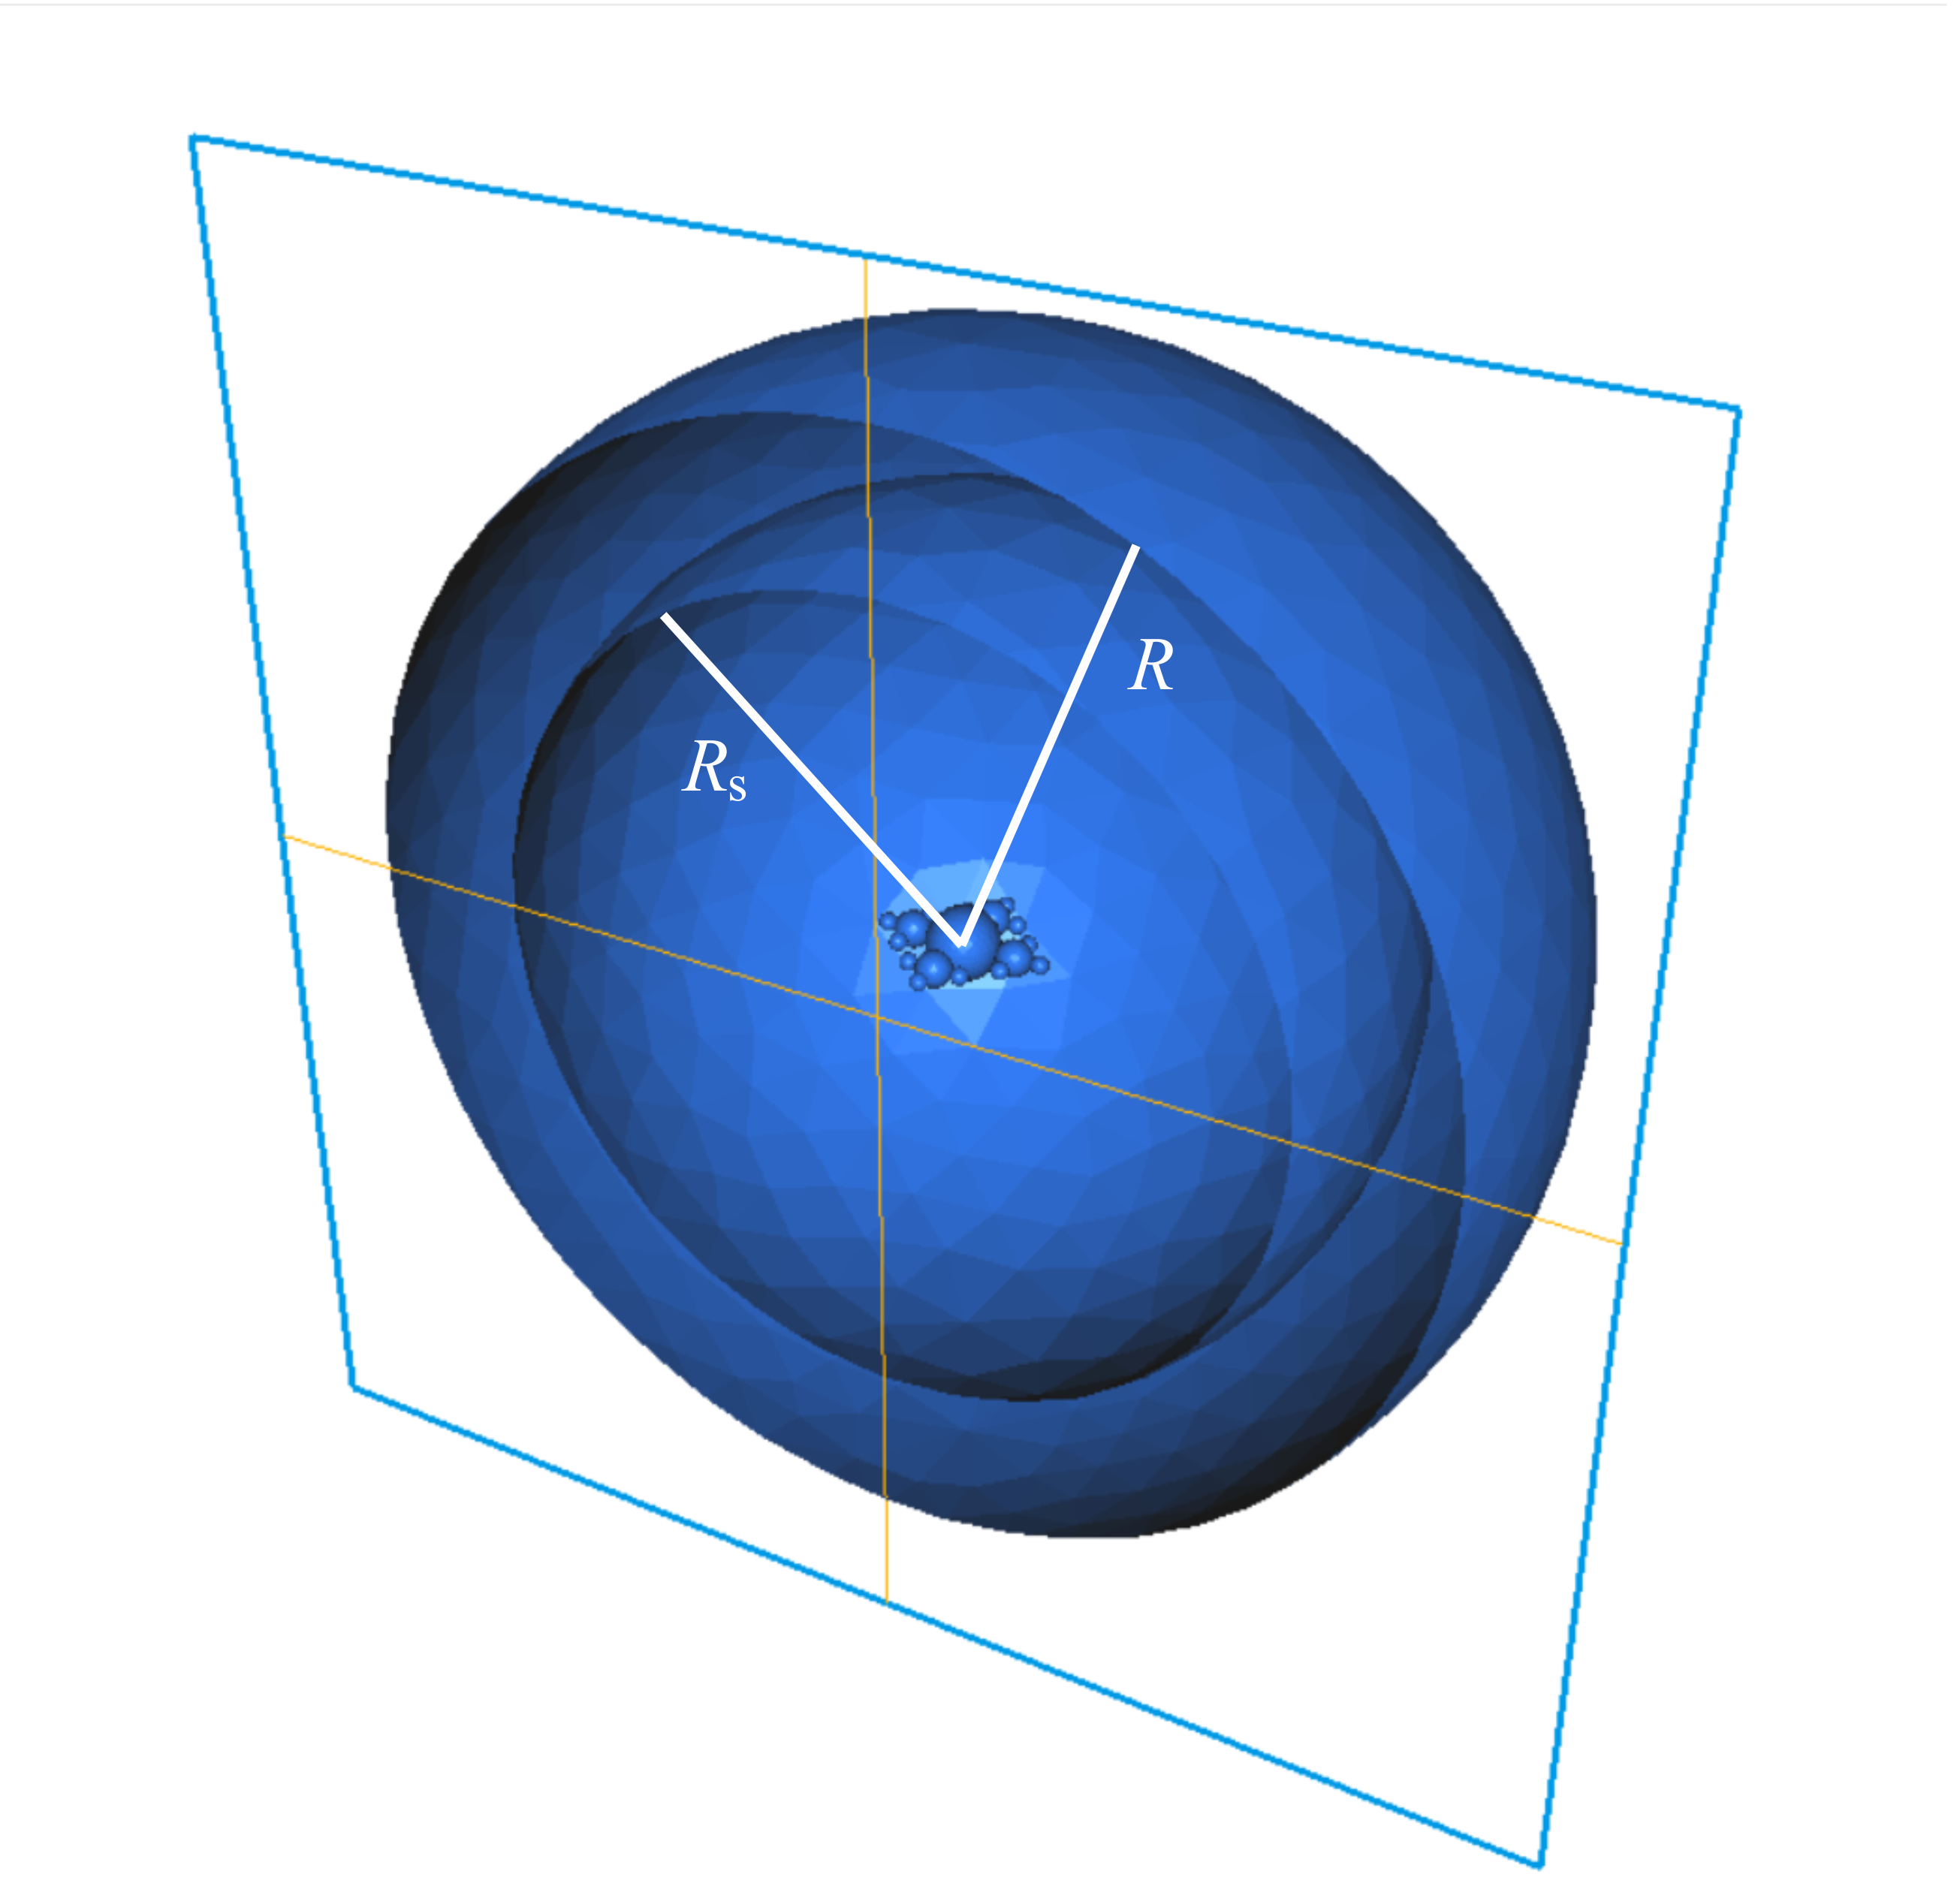
\includegraphics[width=0.6\linewidth]{3td_scattererAndOuterSpheres}
	\caption{}
	\label{fig:3td_scattererAndOuterSpheres}
\end{figure} \\






\subsection{Численная схема и точное решение задачи рассеяния на проводящем цилиндре}
Выведем уравнения для отыскания рассеянного поля при рассеянии плоской волны $H$--- поляризации на идеально-проводящем цилиндре для дальнейшего сравнения с точным решением.

Запишем уравнение Гельмгольца:
\begin{equation}
\Delta H_{z} + k^2H_{z} = 0
\end{equation}
Из уравнений Максвелла получим выражение для $\vec{E}$:
\begin{equation}
	\vec{E} = - \dfrac{i}{k_{0}} {\rm rot}\vec{H} = - \dfrac{i}{k_{0}} \left({\vec x}_{0}\dfrac{\partial {H_{z}}}{\partial y} - {\vec y}_{0}\dfrac{\partial {H_{z}}}{\partial x}\right)
\end{equation}
А так же для $ E_{x}$ и $E_{y} $ соответственно:
\begin{align}
	&E_{x} = - 
	\dfrac{i}{k_{0}}
	\dfrac{\partial{H_{z}}}{\partial y} \\
	&E_{y} = \dfrac{i}{k_{0}}
	\dfrac{\partial{H_{z}}}{\partial x}
\end{align}
Для условной поверхности S : \\
\begin{equation}
[\vec{n}, \vec{x_{0}}E_{x} + \vec{y_{0}}E_{y}] = 0
\end{equation}
Таким образом получим следующее представление:
\begin{equation}
	\int\limits_{V}^{} \Delta H_{z} \cdot wdv = - \int\limits_{V}^{}(\nabla H_{z}, \nabla w)dv +  \int\limits_{V}^{}(\nabla H_{z} \cdot w)dv
\end{equation}
Так как один из интегралов правой части соответственно равен нулю: 
\begin{equation}
	\int\limits_{V}^{}(\nabla H_{z} \cdot w)dv = \oint\limits_{S}^{} \nabla H_{z}  wds \cdot \vec{n} = 0,
\end{equation}
то граничные условия в нашей задаче задавать нет необходимости.
Поэтому получим:
\begin{equation}
	\nabla H_{z} = \vec{x}_{0} \dfrac{\partial H_{z}}{\partial x} - \vec{y}_{0}
	\dfrac{\partial H_{z}}{\partial y}
\end{equation}
Cоответственно используя нормали $n_{x}$ и $n_{y}$  запишем искомое уравнение:
\begin{equation}
	\vec{n}\nabla H_{z} = \dfrac{\partial H_{z}}{\partial n} = 
	n_{x}\dfrac{\partial H_{z}}{\partial x} +
	n_{y}\dfrac{\partial H_{z}}{\partial y}
\end{equation}
Теперь решим ту же самую задачу, но уже точным методом. Для этого в начале найдем уравнения, которые нам понадобятся для решений используя функцию Бесселя $m$-го порядка:
\begin{align}
	&\vec{H} = \vec{r_{0}}H_{z}
	 = e^{-ik_{0}x} = e^{-ik_{0}\rho \rm cos\varphi} = 
	\sum\limits_{m=-\infty}^{\infty} J_{m}(k_{0}\rho)e^{-im(\varphi + \dfrac{\pi}{2})} =\notag\\
	&= \sum\limits_{m=-\infty}^{\infty} (-i)^{m}J_{m}(k_{0}\rho)e^{-im\varphi}.
\end{align}
Запишем уравнение Гельмгольца и оператор Лапласа в следующем виде:
\begin{center}
	$ 
	\Delta_{\perp}H_{z} + k_{0}H_{z} = 0, \qquad
	\Delta_{\perp} = \dfrac{1}{\rho}
	\dfrac{\partial}{\partial \rho} 
	\left(\rho \dfrac{\partial}{\partial \rho}\right) + 
	\dfrac{1}{\rho^{2}}
	\dfrac{\partial^{2}}{\partial \varphi^{2}} .
	$
\end{center}
Получим:
\begin{equation}
	\dfrac{\partial^{2}}{\partial \rho^{2}}H_{z}  +
\dfrac{1}{\rho}\dfrac{\partial}{\partial \rho}H_{z} +
\dfrac{1}{\rho^{2}}\dfrac{\partial^{2}}{\partial \varphi^{2}}H_{z}+
k_{0}^{2}H_{z} = 0.
\end{equation}
Представим $ H_{z} $ как некую $ R(\rho) $ и $ \Phi(\varphi) $:\quad
$ H_{z} = R(\rho)\Phi(\varphi) $, \qquad тогда :
\begin{align}
&\Phi^{\prime\prime}(\varphi) + m^2\Phi(\varphi) = 0,\notag\\ 
&\Phi(\varphi) = e^{-im\varphi},\notag\\
&R^{\prime\prime}(\rho) + \dfrac{1}{\rho} R^{\prime} + (k_{0}^{2} - \dfrac{m^{2}}{\rho^{2}})R = 0.
\end{align}
Используя функцию Ханкеля $m$-го порядка получим, что :
\begin{equation}
	R(\rho) = A_{1}H_{m}^{(1)}(k_{0}\rho) + A_{2}H_{m}^{(2)}(k_{0}\rho).
\end{equation}
Однако  $ A_{1} = 0 $, так как
$\quad \lim\limits_{\rho -> \infty}\sqrt{\rho}
(\dfrac{\partial H_{m}^{(2)}}{\partial \varphi \rho} + ik_{0}H_{m}^{(1)} ).
$ 
В таком случае у нас остается:
$$
H_{z} = \sum_{m=-\infty}^{\infty}A_{2m}H_{m}^{(2)}(k_{0}\rho)e^{-im\varphi}
$$
\\
Граничные условия:
\begin{equation}
	E_{\varphi}|_{\rho=a} = 0
\end{equation}
Тогда:
\begin{eqnarray}
&&\vec{E}^{(s)} = - \dfrac{i}{k_{0}\varepsilon} {\rm rot}\vec{H}^{(s)} = - \dfrac{i}{k_{0}} \dfrac{1}{\rho}
\begin{vmatrix}
\vec{\rho}_{0}& \;\rho \vec{\varphi}_{0}& \; \vec{z}_{0} \\
\dfrac{\partial }{\partial \rho}& \; 
\dfrac{\partial }{\partial \varphi}&\; 
\dfrac{\partial }{\partial z} \\
H_{\rho}^{(s)}&\; \rho H_{\varphi}^{(s)}&\; H_{z}^{(s)}
\end{vmatrix}
=\notag\\
&& = \dfrac{i}{k_{0}} \dfrac{1}{\rho}\left(\vec{\rho}_{0}
\dfrac{\partial H_{z}}{\partial \rho} - \rho\vec{\varphi}_{0}
\dfrac{\partial H_{z}^{(s)}}{\partial \rho}\right),
\\
&&E_{\varphi}^{(s)} = \dfrac{i}{k_{0}}
\dfrac{\partial }{\partial \rho} \sum_{m=-\infty}^{\infty} A_{2m}H_{m}^{(2)}(k_{0}\rho)e^{-im\varphi} = i\sum_{m=-\infty}^{\infty}A_{2m}{H_{m}^{(2)}}^{\prime}(k_{0}\rho)e^{-im\varphi}.
\end{eqnarray}
Исходя из граничных условий для падающей и отраженной волны:
\begin{align}
&E_{\varphi}|_{\rho=a} = (E_{\varphi}^{(i)} + E_{\varphi}^{(s)})|_{\rho=a},\notag\\ &\sum_{m=-\infty}^{\infty}
((-i)^{m}J_{m}^{\prime}(k_{0}\rho) + A_{2m}{H_{m}^{(2)}}^{\prime}(k_{0}\rho))e^{-im\varphi}|_{\rho=a} = 0.
\end{align}
Получим искомое выражение:
\begin{align}
&(-i)^{m}J_{m}^{\prime}(k_{0}a) + A_{2m}{H_{m}^{(2)}}^{\prime}(k_{0}a) = 0,\\
&A_{2m} = (-i)^{m} \dfrac{J_{m}^{\prime}(k_{0}a)}
{{H_{m}^{(2)}}^{\prime}(k_{0}a)}.
\end{align}


\section{Тестирование численной схемы}
Для проведения численных расчётов будем использовать пакет программ FreeFem++ \cite{bfreefem}.

Приступим к созданию трехмерной модели в программе FreeFem++ на основе полученных нами выше выражений \cite{bfreefem}.  Для этого выберем наиболее подходящий программный способ реализации 3D объектов, а так же сразу определим, что наш объект будет в виде шаров (у которых тут же зададим радиус и другие параметры). Возьмем сферическую область, в которой будут рассеиваться волны и заключим в нее наш объект - сферу более маленького радиуса заполненного диэлектриком.
Определим параметры характеризующие наше поле,а именно:
	$ \lambda$ - длина волны в вакууме в метрах,
	$ c = 299792458 $ - скорость света в вакууме, $ n$ - показатель преломления среды шаров.
Выберем один из способов аппроксимации функций для метода конечных элементов, заложенных в программе: P0 - кусочно-постоянные разрывные функции, P1 - кусочно-линейно непрерывные функции, P2 - кусочно-непрерывные(гладкие) функции (аппроксимация полиномами 2го порядка), так же в программе есть их разновидности (P1c, P1b, P2dc и т.д.), которые мы рассматривать не будем. Для нахождения рассеяния на цилиндре будем использовать P2, ввиду более точных результатов, в остальных случаях P1 для ускорения расчетов.\\
При всех вычислениях радиус наибольшего внутреннего шара зададим в 10 раз меньшим длины волны принимаемой для расчетов, а радиус внешней сферы в 4 раза больше длины волны. Таким образом получим систему состоящую из двух сфер разного радиуса (одна внутри другой), взаимодействие между которыми опиcываются с помощью уравнений полученных ранее. Однако, прежде чем мы это сделаем, определим в программе область расчетов через радиус внутренней сферы, для случаев когда он больше или меньше радиуса применяемого для вычислений полей в ближней и дальней зоне. Необходимость этого заключается в том, что уравнение должно выполняться для каждого из малых объемов, а не в каждой точке, как было сказано ранее.
\\
Определим k для случаев:
\begin{equation}
	k = 
	\begin{cases}
		1, & r > a\\
		n, & r < a ,\qquad \text{где }a \text{ --- радиус малой сферы}
	\end{cases}
\end{equation}
Далее добавим цикл, который ввиду гармонической зависимости от времени будет производить перерасчет данных и выводить результаты на экран, благодаря чему получится наглядная анимированная картина поля. А также добавим возможность сохранения полученных данных для Matlab. После того, как мы посчитали дифракцию на сфере, перейдем непосредственно к расчету сечения рассеяния и сечения поглощения. Если на рассеивающий элемент падает волна с интенсивностью I(под интенсивностью понимается поток энергии через единичную площадку), то полная рассеянная мощность S будет пропорциональна I. Коэффициент пропорциональности между этими величинами $ \sigma_s $ называется полным сечением рассеяния и имеет размерность площади:
\begin{equation}
	\sigma_s = \dfrac{S}{I} 
\end{equation}
Так же введем понятие дифференциального сечения рассеяния
 $ \sigma_d(\theta,\varphi) $. Пусть $ dS(\theta, \varphi) $ - полная мощность, рассеянная в пределах телесного угла d$ \Omega $ в направлении $ (\theta,\varphi) $, тогда:
 \begin{center}
 	$ \sigma_d(\theta,\varphi) = \lim\limits_{d\Omega\rightarrow\infty} \dfrac{dS(\theta, \varphi)}{Id\Omega}. $
 \end{center}
Применительно к нашей задаче, это выражение примет вид:
\begin{equation}
\sigma_d(\theta,\varphi) = \lim\limits_{R\rightarrow\infty} \dfrac{R^2 S_r(\theta, \varphi)}{S_i}.
\end{equation}
Здесь средний за период колебания поля вектор Пойнтинга падающей волны
\begin{equation}
{\vec S}_i = \dfrac{c}{8\pi} {\rm Re} \left[{\vec E}_i \times {\vec H}^*_i\right],
\end{equation}
радиальная компонента вектора Пойнтинга рассеянных волн
\begin{equation}
{S}_r = \dfrac{c}{8\pi} {\rm Re} \left[{\vec E}_s \times {\vec H}^*_s\right] \cdot {\vec \rho}_0
\end{equation}
В нашем случае при расчётах необходимо будет взять значения вектора Пойнтинга рассеянных волн на поверхности с фиксированным значением $R$ (приемлемо, если $R=3\lambda$, т.к. внешняя граница удалена на расстояние $4\lambda$).\\
Наиболее простой способ расчёта $S_r$ через компоненты в декартовой системе координат:
\begin{equation}
{S}_r = S_x {\rm cos}(\varphi)\sin(\theta) + S_y \sin(\varphi)\sin(\theta) + S_z {\rm cos}(\theta).
\end{equation}
Здесь
\begin{eqnarray}
& S_x = \dfrac{c}{8\pi} {\rm Re} \left(E_y H_z^* - E_z H_y^*\right),\nonumber\\
& S_y = \dfrac{c}{8\pi} {\rm Re} \left(E_z H_x^* - E_x H_z^*\right),\nonumber\\ & S_z = \dfrac{c}{8\pi} {\rm Re} \left(E_x H_y^* - E_y H_x^*\right).
\end{eqnarray}
Предполагается, что поля относятся к рассеянному полю (индеркс $s$ опущен).
Компоненты магнитного поля находим из уравнения Максвелла
\begin{equation}
{\vec H} = \dfrac{i}{k_0} {\rm \rm rot} \vec{E}.
\end{equation}
Полное сечение рассеяния находится как интеграл по полному телесному углу:
\begin{equation}
\sigma_s = \int_{4\pi} \sigma_d d\Omega.
\end{equation}
Сечение поглощения определяется как отношение полной мощности, теряемой первичной волной и преобразующейся в тепло в данной локальной области, к плотности потока энергии(интенсивности) в первичной волне. Его находим как:
\begin{equation}
\sigma_a = \left(\int_V \dfrac{1}{2}\omega\varepsilon''|{\vec E}|^2 d V\right)/S_i.
\end{equation}
В случае, если падающее поле имеет единичную амплитуду ($|E_i|=1$):
\begin{equation}
\sigma_a = 4\pi \int_V k \varepsilon''|{\vec E}|^2 d V.
\end{equation}
Здесь интегрирование проводится по области занятой диэлектрическим рассеивателем.\\
Вычисление действительной и мнимой частей диэлектрической проницаемости на основе коэффициента преломления будет выглядеть как:
\begin{equation}
\varepsilon' - i \varepsilon'' = (n'-i n'')^2.
\end{equation}
Отсюда действительная $ \varepsilon' $ и мнимая $ \varepsilon'' $ часть будут соответственно равны:
\begin{equation}
\varepsilon' = (n')^2 - (n'')^2,\quad \varepsilon'' = 2 n'n''.
\end{equation}

\section{Результаты численных расчётов}


%Сразу определим, что внутри нашего объекта область заполнена диэлектриком, а его радиус будет в 10 раз меньше длины волны принимаемой для расчетов ($ \lambda = 1 $), а радиус сферической области в 4 раза больше (Рис.\ref{fig:ces1}). Так же стоит отметить, что на протяжении всей работы будет использоваться гармоническая зависимость $ e^{j \omega t} $, где $ j = \sqrt{-1} $. Далее найдем сечение рассеяния $ \sigma_s $ и сечение поглощения $ \sigma_a $, которое будет находиться на удалении $ \lambda = 3 $, с помощью действительной $ \varepsilon' $ и мнимой $ \varepsilon'' $ части диэлектрической проницаемости на основе коэффициентов преломления $ n' $ и $ n'' $.
%

Прежде чем использовать вычислительный пакет программ FreeFem++ для сформулированной задачи, убедимся в точности проводимых расчётов на модельной задаче --- рассеяние на идеально-проводящем цилиндре.
\begin{figure}[h!]
	\centering
	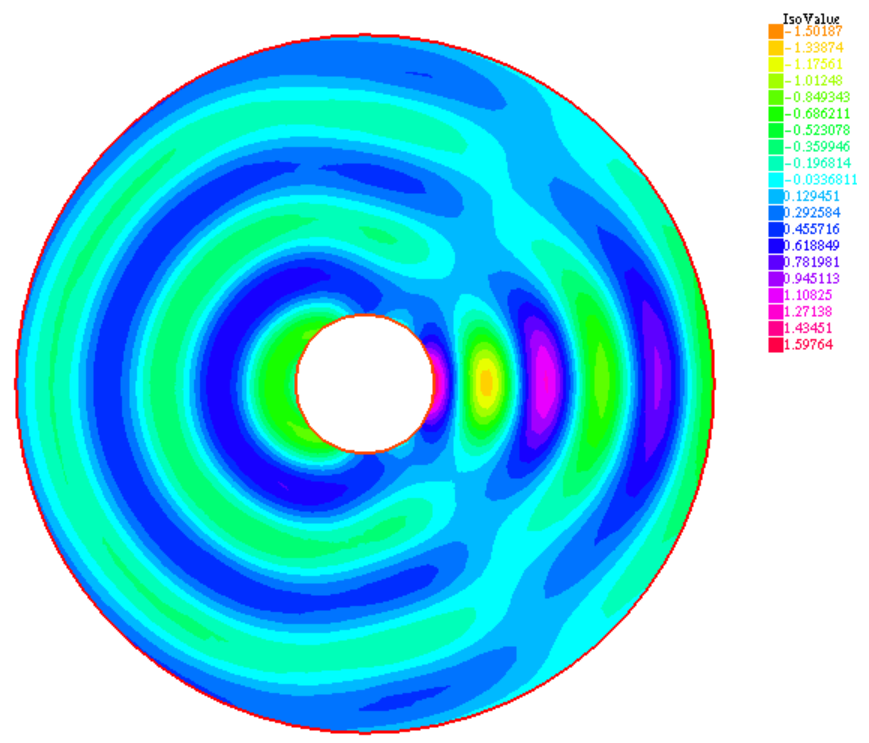
\includegraphics[width=0.8\linewidth]{sc1.png}
	\caption{Численный метод}
	\label{fig:sc1}
\end{figure} 
\newpage
\begin{figure}[h!]
	\centering
	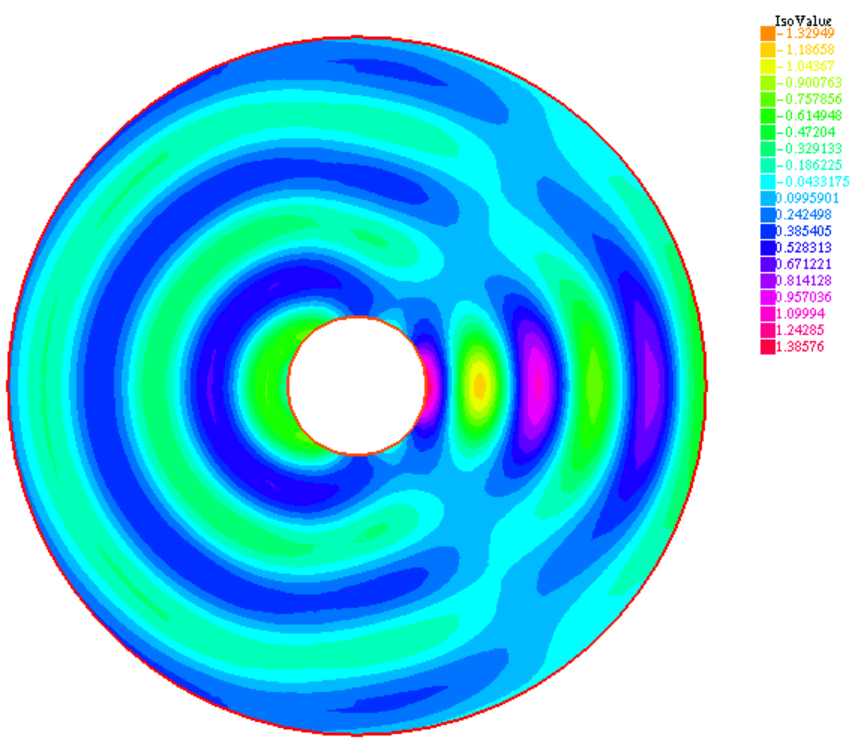
\includegraphics[width=0.8\linewidth]{sc2.png}
	\caption{Точный метод}
	\label{fig:sc2}
\end{figure}
Как видно из Рис. \ref{fig:sc1} и \ref{fig:sc2} при рассеянии плоской волны на цилиндре мы получили практически одинаковые значения поля в точках с точностью до фазы, несмотря на то, что вычисление производилось разными математическими методами, что в свою очередь показывает правильную постановку задачи и ее верное решение. \\ 
Ниже приведены результаты численных расчётов сечения рассеяния и сечения поглощения нормированные на квадрат длины волны в зависимости от длины падающей волны, и состоящие из одного шара, пяти и семнадцати. Шары заполнены золотом \cite{Olmon2012}, серебром \cite{Yang2015}, либо медью \cite{Querry1985}. Для расчетов применяются оптические плотности материалов. Здесь и далее зелёными кривыми отмечены результаты расчётов для золота, синим – серебра, красным – меди.

%С ростом частоты, происходит существенное уменьшению диапазона длин волн как для сечения поглощения (например \ref{fig:singleCopperSphereAbsorptionSection},  \ref{fig:singleSilverSphereAbsorptionSection}, \ref{fig:singleGoldSphereAbsorptionSection}), так и сечения рассеяния (например \ref{fig:singleCopperSphereAbsorptionSection}, \ref{fig:singleSilverSphereAbsorptionSection}, \ref{fig:singleGoldSphereAbsorptionSection}), для которого зависимость будет ближе к гиперболической. В частности графики (Рис. \ref{fig:singleCopperSphereCrossSection}, \ref{fig:singleSilverSphereCrossSection}, \ref{fig:singleGoldSphereCrossSection}) будут напоминать график гиперболического косеканса (Рис. \ref{fig:csch}), причем в дальнейшем при увеличении числа рассеивателей эта зависимость будет сохраняться, в случае с 5 сферами (Рис. \ref{fig:fiveCopperSphereCrossSection}, \ref{fig:fiveSilverSphereCrossSection}, \ref{fig:fiveGoldSphereCrossSection}) или 17 сферами (Рис. \ref{fig:seventeenCopperSphereCrossSection}, \ref{fig:seventeenSilverSphereCrossSection}, \ref{fig:seventeenGoldSphereCrossSection}). Получается, что для рассеяния волны требуется высокая частота, но лишь в ограниченном диапазоне длин волн, так как добиться отрицательного коэффициента преломления, можно лишь когда диэлектрическая проницаемость и магнитная восприимчивость так же будут отрицательными, однако верно это будет в небольшом диапазоне длин волн, что подтверждается теорией фрактальных антенн и метаматериалов представленной ранее. И если со вторым все более-менее понятно, то как можно объяснить требования высокой частоты? Чтобы добиться отрицательной реакции, необходимо подбирать частоты колебаний при использовании резонансной характеристики среды таким образом, чтобы силы, создаваемые электрическими и магнитными полями, воздействовали в противоположном направлении движению электронов. Так, если толкнуть качели, то они начнут двигаться с частотой собственных колебаний и подталкивая их с этой частотой мы будем входить в резонанс, тем самым увеличивать амплитуду. Если же мы начнем толкать их с более высокой частотой, то в какой-то момент наши толчки перестанут совпадать с колебаниями по фазе и рука ударится о движущиеся ей навстречу качели. Похожим образом ведут себя электроны, входящие в противофазу и начинающие сопротивляться "толчкам" электромагнитного поля.
%Увеличение элементов рассеивателя приводит расширению диапазона длин волн для сечения поглощения с одиночной сферой (Рис.\ref{fig:singleCopperSphereAbsorptionSection},\ref{fig:singleGoldSphereAbsorptionSection}),5 сферами (Рис.\ref{fig:fiveCopperSphereAbsorptionSection},\ref{fig:fiveGoldSphereAbsorptionSection}), и 17 сферами (Рис.\ref{fig:seventeenCopperSphereAbsorptionSection},\ref{fig:seventeenGoldSphereAbsorptionSection}) в случае если материал – медь и в меньшей степени если это золото, однако с каждой новой итерацией изменение менее значительно. Тоже самое нам говорит теория фрактальных антенн, увтерждающая, что весомый вклад вносят лишь пара первых итераций, которые называют кривыми, заполняющие пространство (Space Filling Curve) \cite{b12}\cite{b13}, а дальнейшее увеличение элементов не даст столь значительного эффекта.  В случае с серебром (Рис.\ref{fig:singleSilverSphereAbsorptionSection},\ref{fig:fiveSilverSphereAbsorptionSection},\ref{fig:seventeenSilverSphereAbsorptionSection}), это изменение очень мало и заметно лишь через одну итерацию. Для сечения рассеяния увеличение числа элементов существенных изменений не вносит. Так же стоит помнить, что уменьшая размер антенны (каждая новая итерация сфер меньше предыдущей в 2 раза), мы уменьшаем длину волны, для которой среда будет иметь отрицательный показатель преломления. \\
%Изменение материала рассеивателя приводит к изменению максимальной частоты и расширению/сужению диапазона длин волн в зависимости от того, какой материал был выбран. Так же исходя из теории стоит помнить, что чем больше мощности первичной волны будет поглощено в сечении поглощении материала, тем больше его будет преобразовано в тепло. Конечно, речь не идет о каких-то больших значениях, однако этот факт тоже стоит иметь ввиду.
%Из графиков (Рис. \ref{fig:singleCopperSphereAbsorptionSection} и \ref{fig:singleSilverSphereAbsorptionSection}, \ref{fig:fiveCopperSphereAbsorptionSection} и \ref{fig:fiveSilverSphereAbsorptionSection}, \ref{fig:seventeenCopperSphereAbsorptionSection} и \ref{fig:seventeenSilverSphereAbsorptionSection}) видно, что большее поглощение происходит на медной сфере, а меньшее на серебряной. Золотая сфера в это случае занимает промежуточную позицию. В случае с сечением рассеяния (Рис. \ref{fig:singleCopperSphereCrossSection} и \ref{fig:singleGoldSphereCrossSection}, \ref{fig:fiveCopperSphereCrossSection} и \ref{fig:fiveGoldSphereCrossSection}, \ref{fig:seventeenCopperSphereCrossSection} и \ref{fig:seventeenGoldSphereCrossSection}) медь и золото демонстрируют почти одинаковые результаты, однако у первого материала максимальная частота не много выше, серебро же (Рис. \ref{fig:singleSilverSphereCrossSection}, \ref{fig:fiveSilverSphereCrossSection}, \ref{fig:seventeenSilverSphereCrossSection}) показывает гораздо меньшие результаты. \\
%Из всего вышеперечисленного, можно сделать вывод, что для работы на более высоких частотах необходимо использовать более короткие длины волн определенного диапазона, а так же подбирать частоту колебаний при использовании резонансной характеристики среды. Для работы же на более длинных волнах требуется увеличить количество элементов рассеивателя или изменить материал, из которого они состоят.
Как можно видеть, увеличение сложности конфигурации рассеивателя приводит к возрастанию как сечения поглощения  (Рис. \ref{fig:absorpForONE}, \ref{fig:absorpForFIVE}, \ref{fig:absorpForSEVENTEEN}), так и сечения рассеяния (Рис. \ref{fig:scatForONE}, \ref{fig:scatForFIVE}, \ref{fig:scatForSEVENTEEN}). Это лучше всего
просматривается при сравнении одиночного шара и рассеивателя «первой итерации», однако с каждой последующей итерацией это изменение менее значительно. Разница между приведёнными величинами для рассеивателя «первой итерации» (Рис. \ref{fig:absorpForFIVE} и \ref{fig:scatForFIVE}) и рассеивателя «второй итерации» (Рис. \ref{fig:absorpForSEVENTEEN} и \ref{fig:scatForSEVENTEEN}) не столь ярко выражена. При этом, как сечение поглощения, так и сечение рассеяния будут наименьшие для рассеивателей, составленных из серебра.
 
Кроме того, из полученных графиков видно, что увеличение сложности рассеивателя приводит к увеличению сечения рассеяния для всех сред и всех длин волн (Рис. \ref{fig:scatForCopper}, \ref{fig:scatForSilver}, \ref{fig:scatForGold}), за исключением небольшого интервала в оптической области частот для серебряных рассеивателей в котором семнадцать шаров имеют меньшее сечение рассеяния, чем пять шаров (Рис. \ref{fig:scatForSilver}). В тоже время, сечения поглощения для всех материалов в инфракрасной области частот возрастает с увеличением числа элементов рассеивателя, а в оптической области сечение поглощения рассеивателя «второй итерации» уменьшается по сравнению с сечением поглощения рассеивателя «первой итерации»(Рис. \ref{fig:absorpForCopper}, \ref{fig:absorpForSilver}, \ref{fig:absorpForGold}).
При этом, как видно из рисунков для серебра и золота, локальный минимум зависимости сечения поглощения от длины волны смещается в сторону больших длин волн с увеличением сложности рассеивателя.
Из всего вышеперечисленного, можно сделать вывод, что для работы на более высоких частотах необходимо использовать более короткие длины волн определенного диапазона. Для работы же на более длинных волнах требуется увеличить количество элементов рассеивателя или изменить материал, из которого они состоят.\\

\begin{figure}[h!]
	\centering
	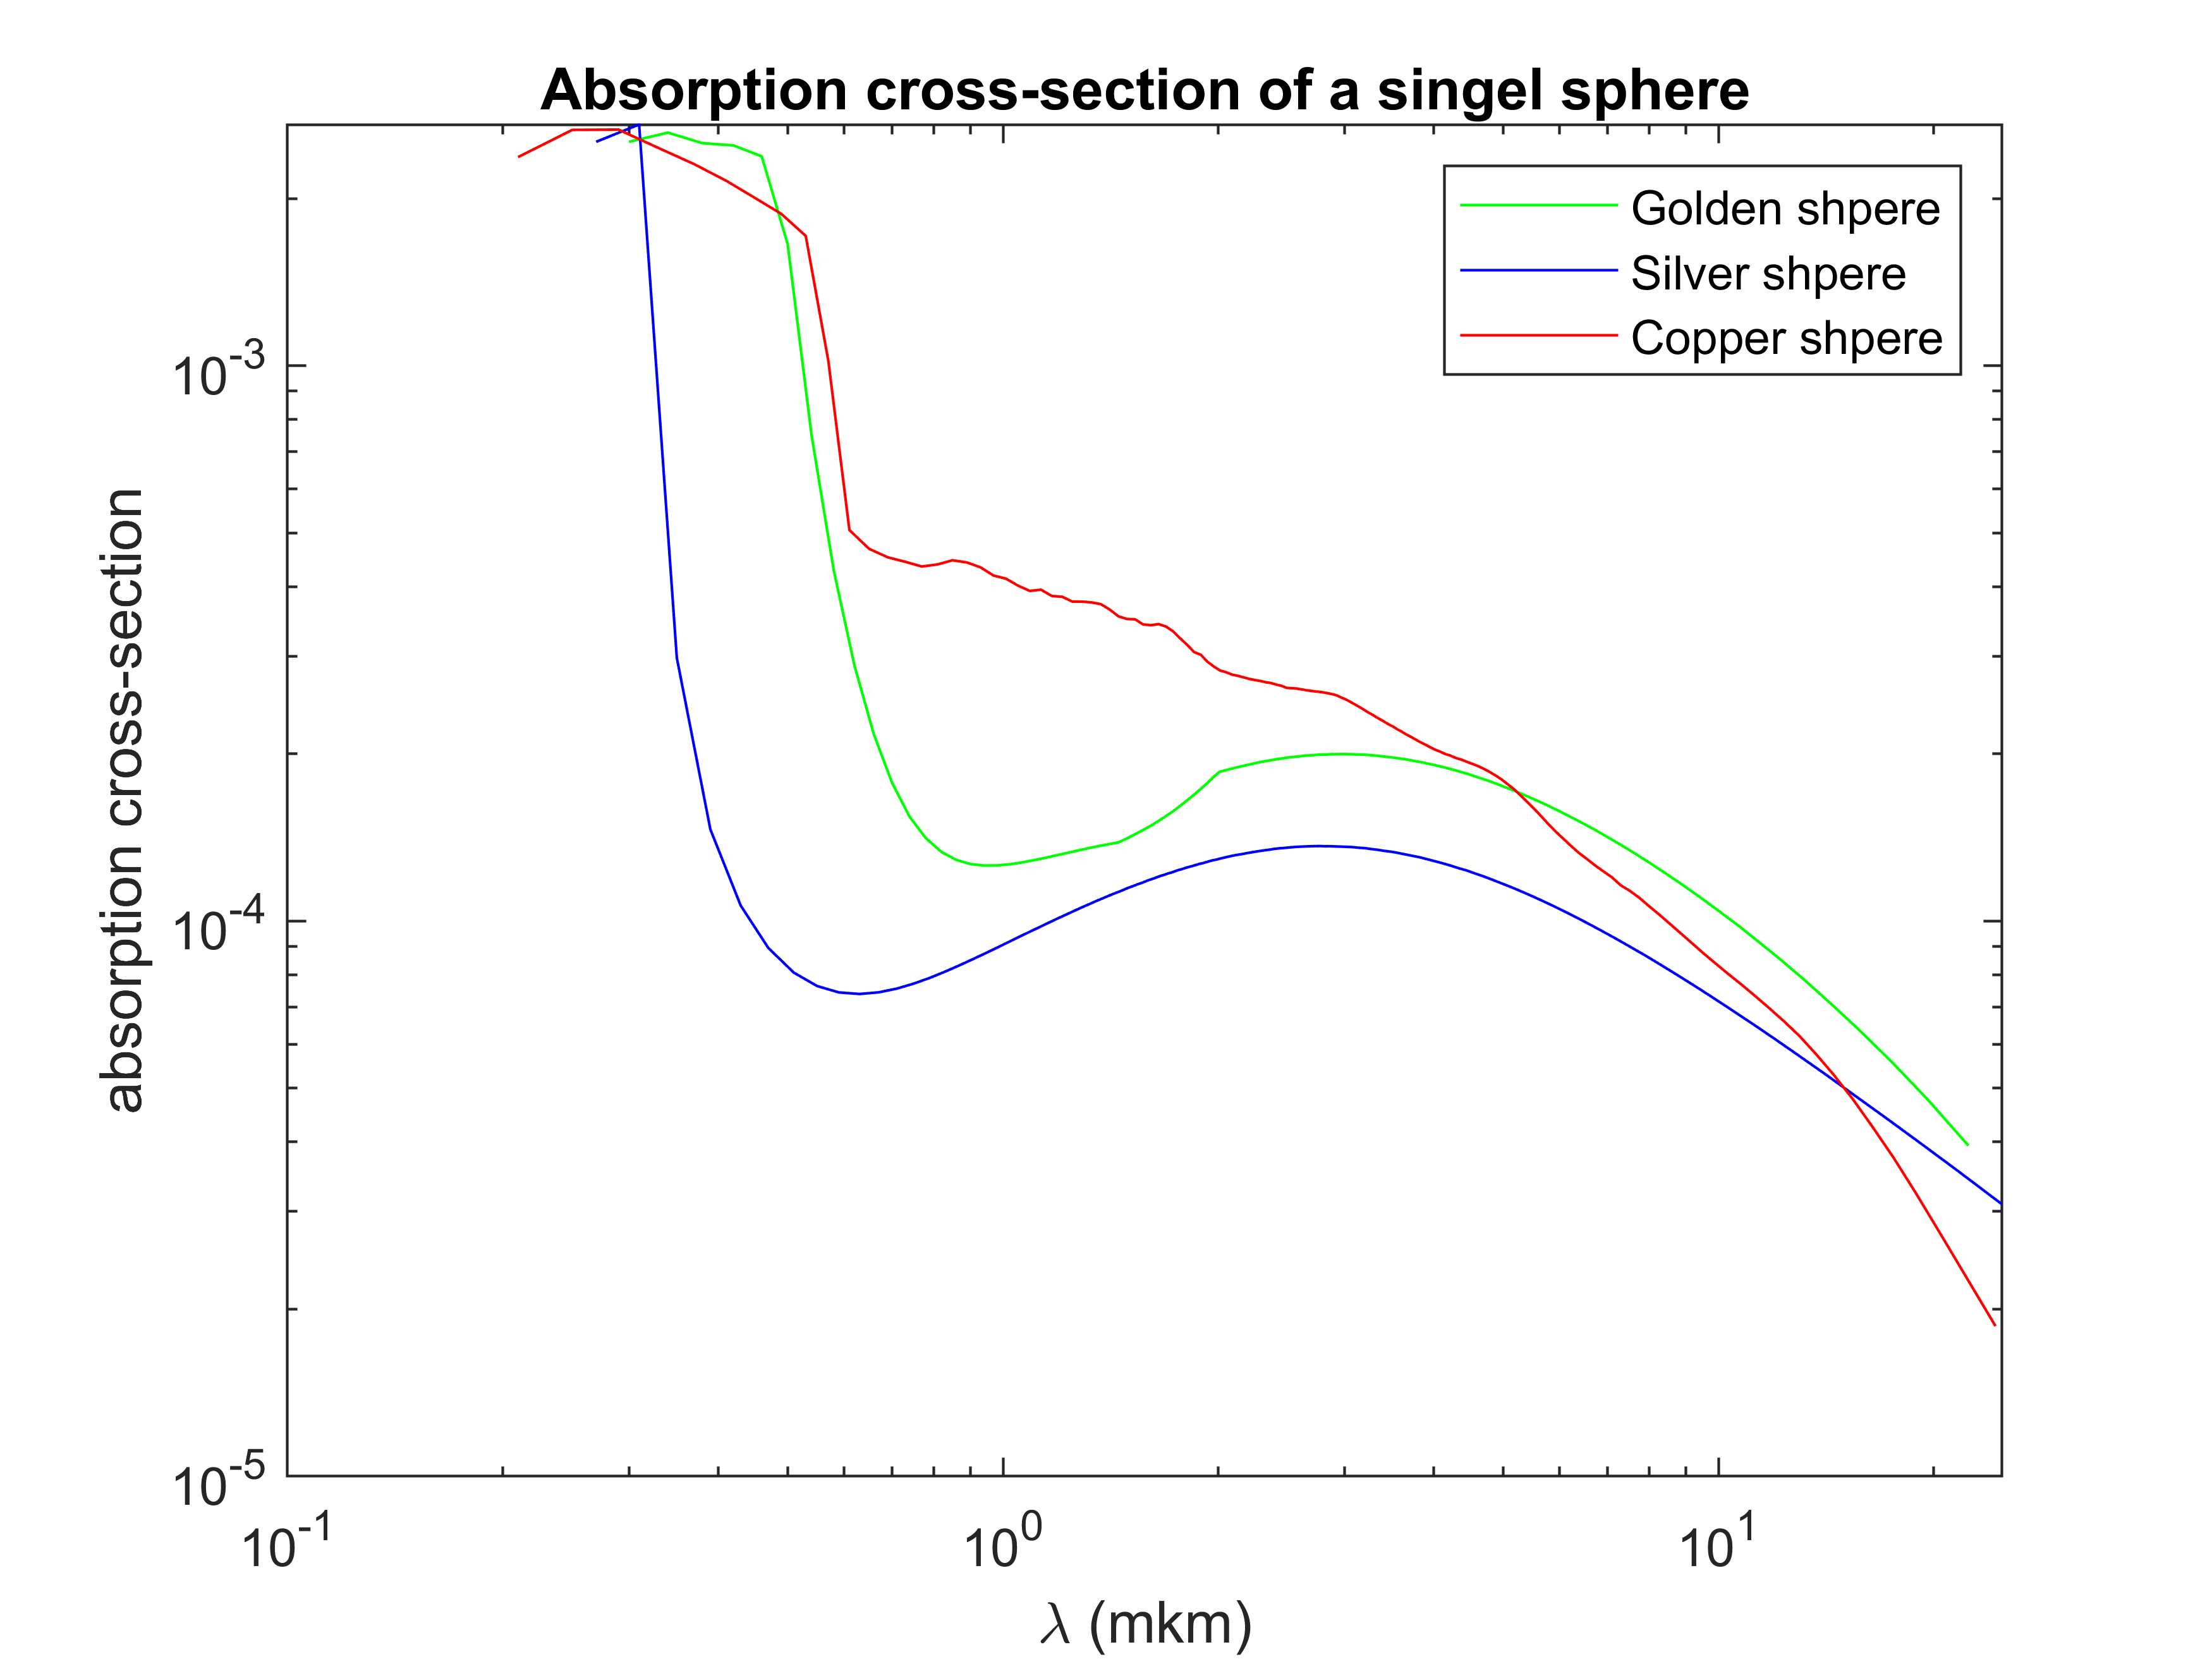
\includegraphics[width=0.8\linewidth]{absorpForONE}
	\caption{Сечение поглощения для одного шара в разных средах}
	\label{fig:absorpForONE}
\end{figure} 
\begin{figure}[h!]
	\centering
	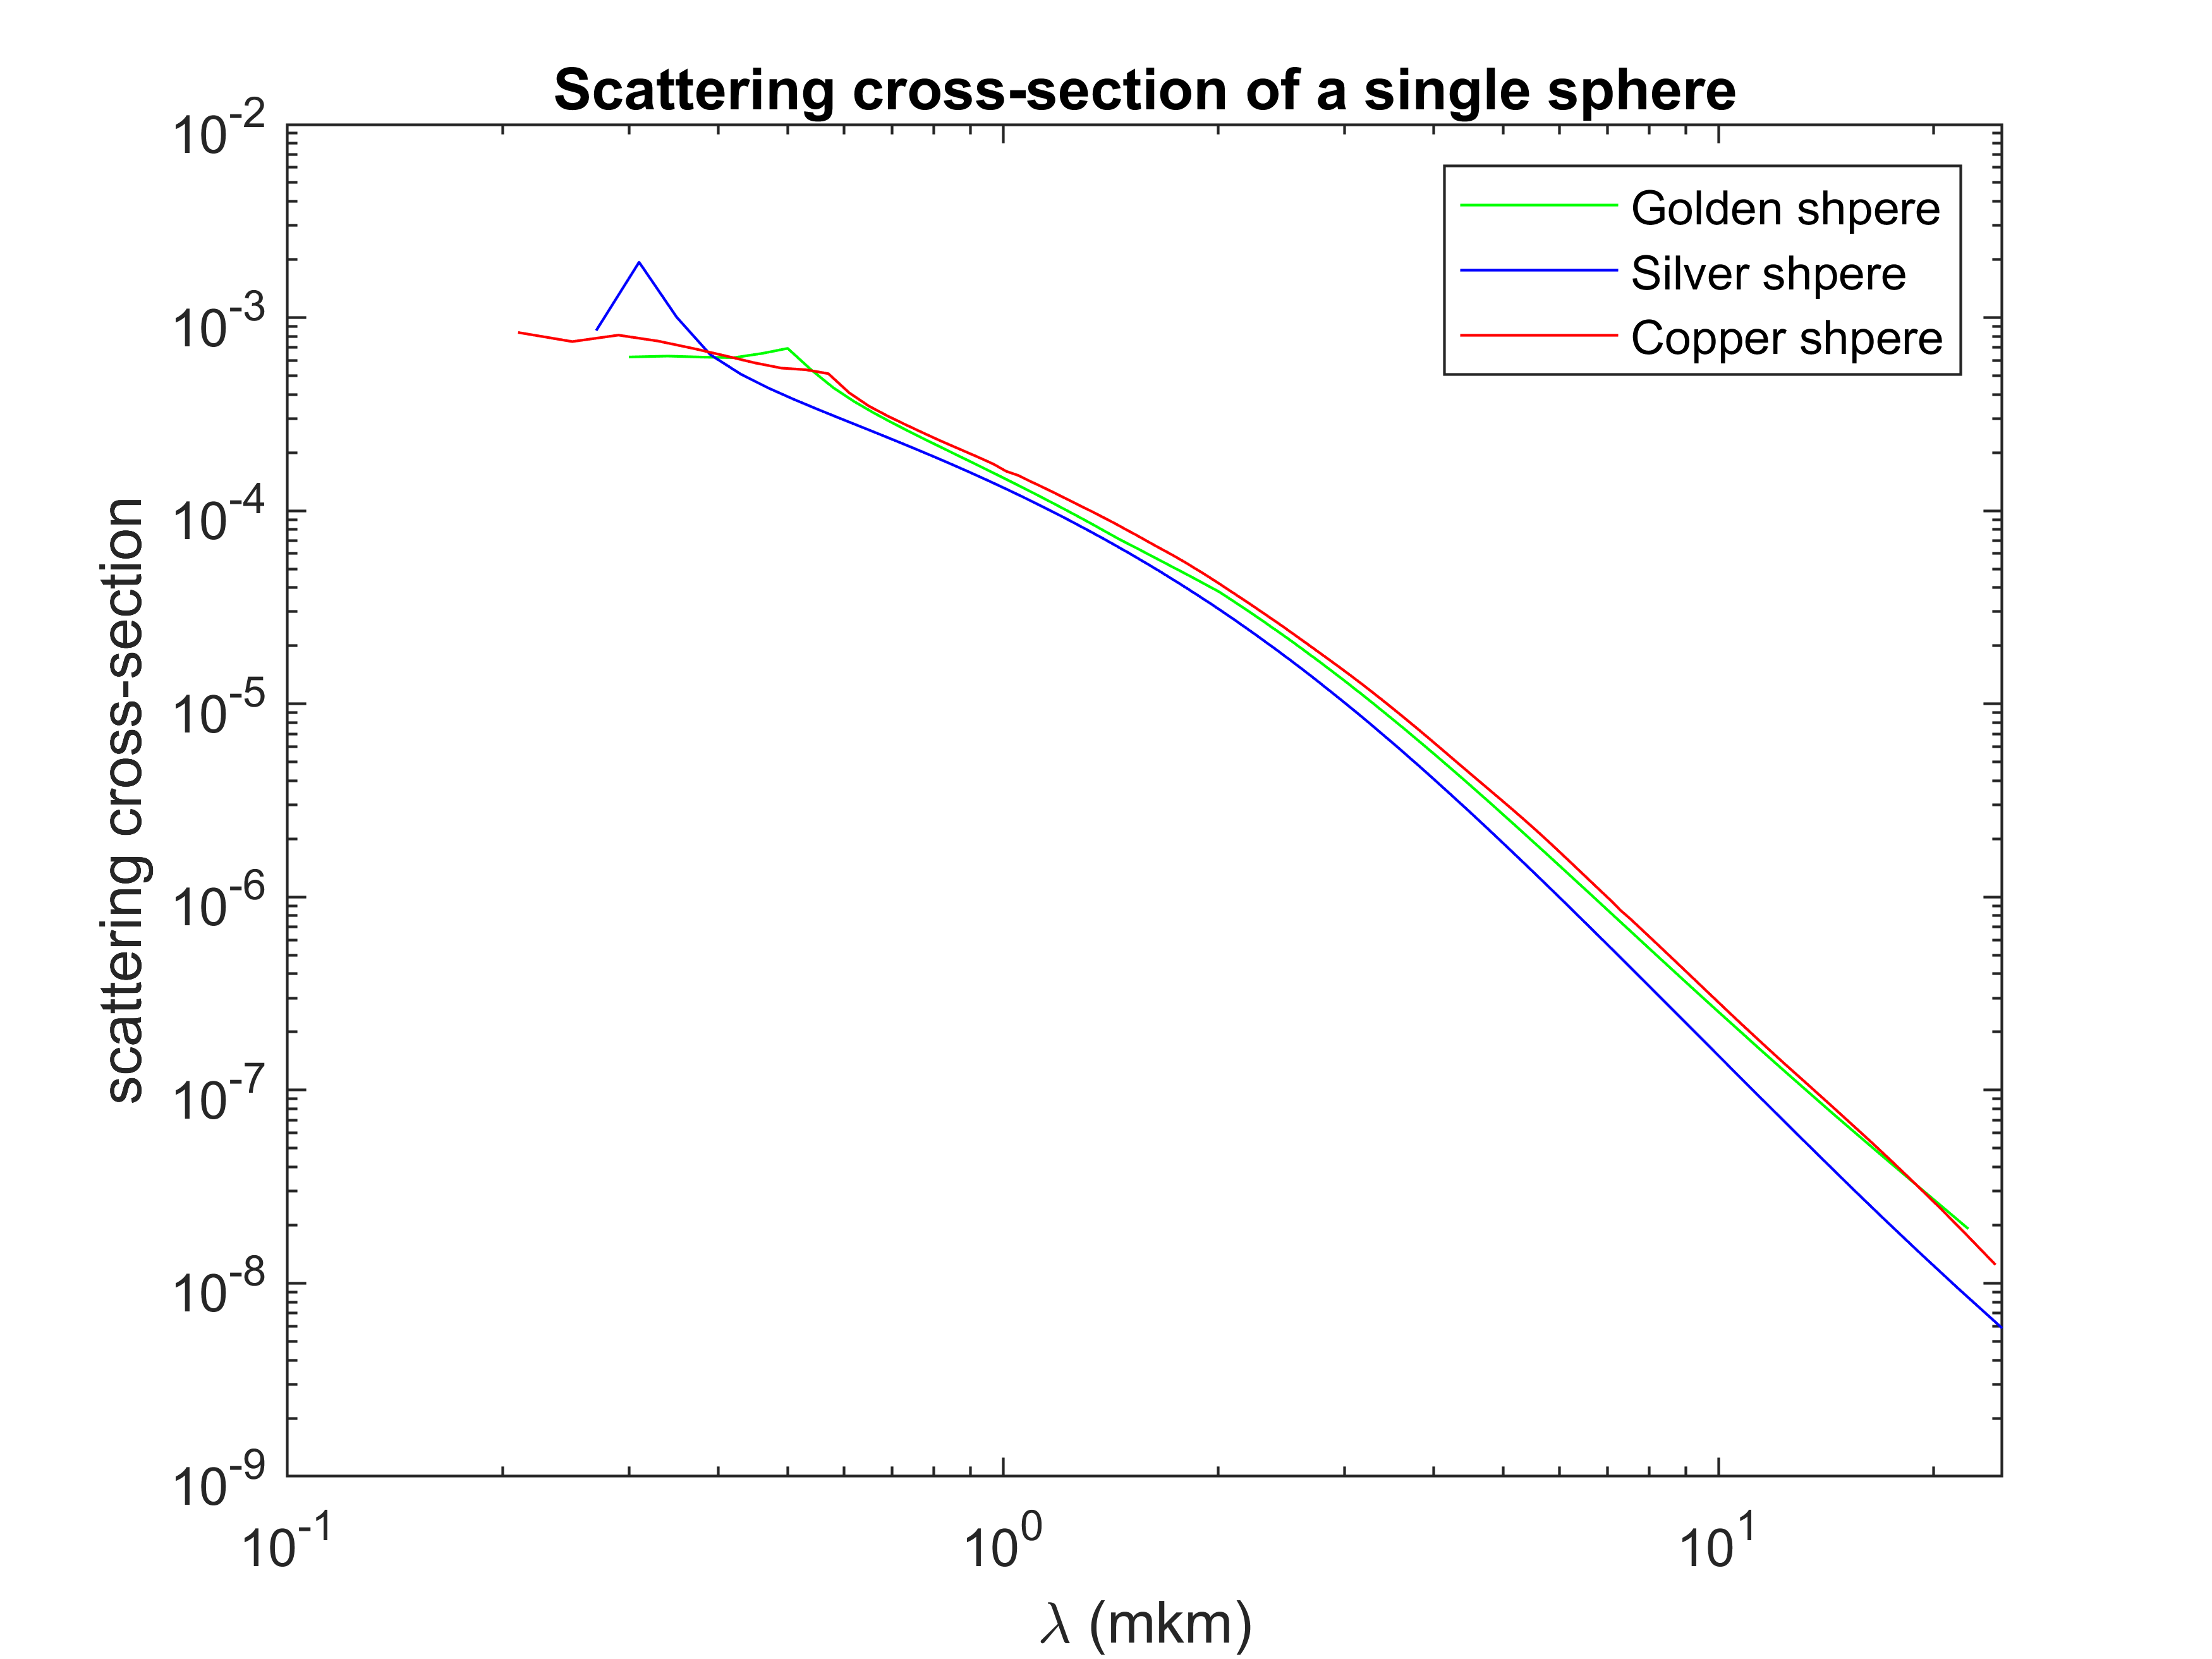
\includegraphics[width=0.8\linewidth]{scatForONE}
	\caption{Сечение рассеяния для одного шара в разных средах}
	\label{fig:scatForONE}
\end{figure} 
\begin{figure}[h!]
	\centering
	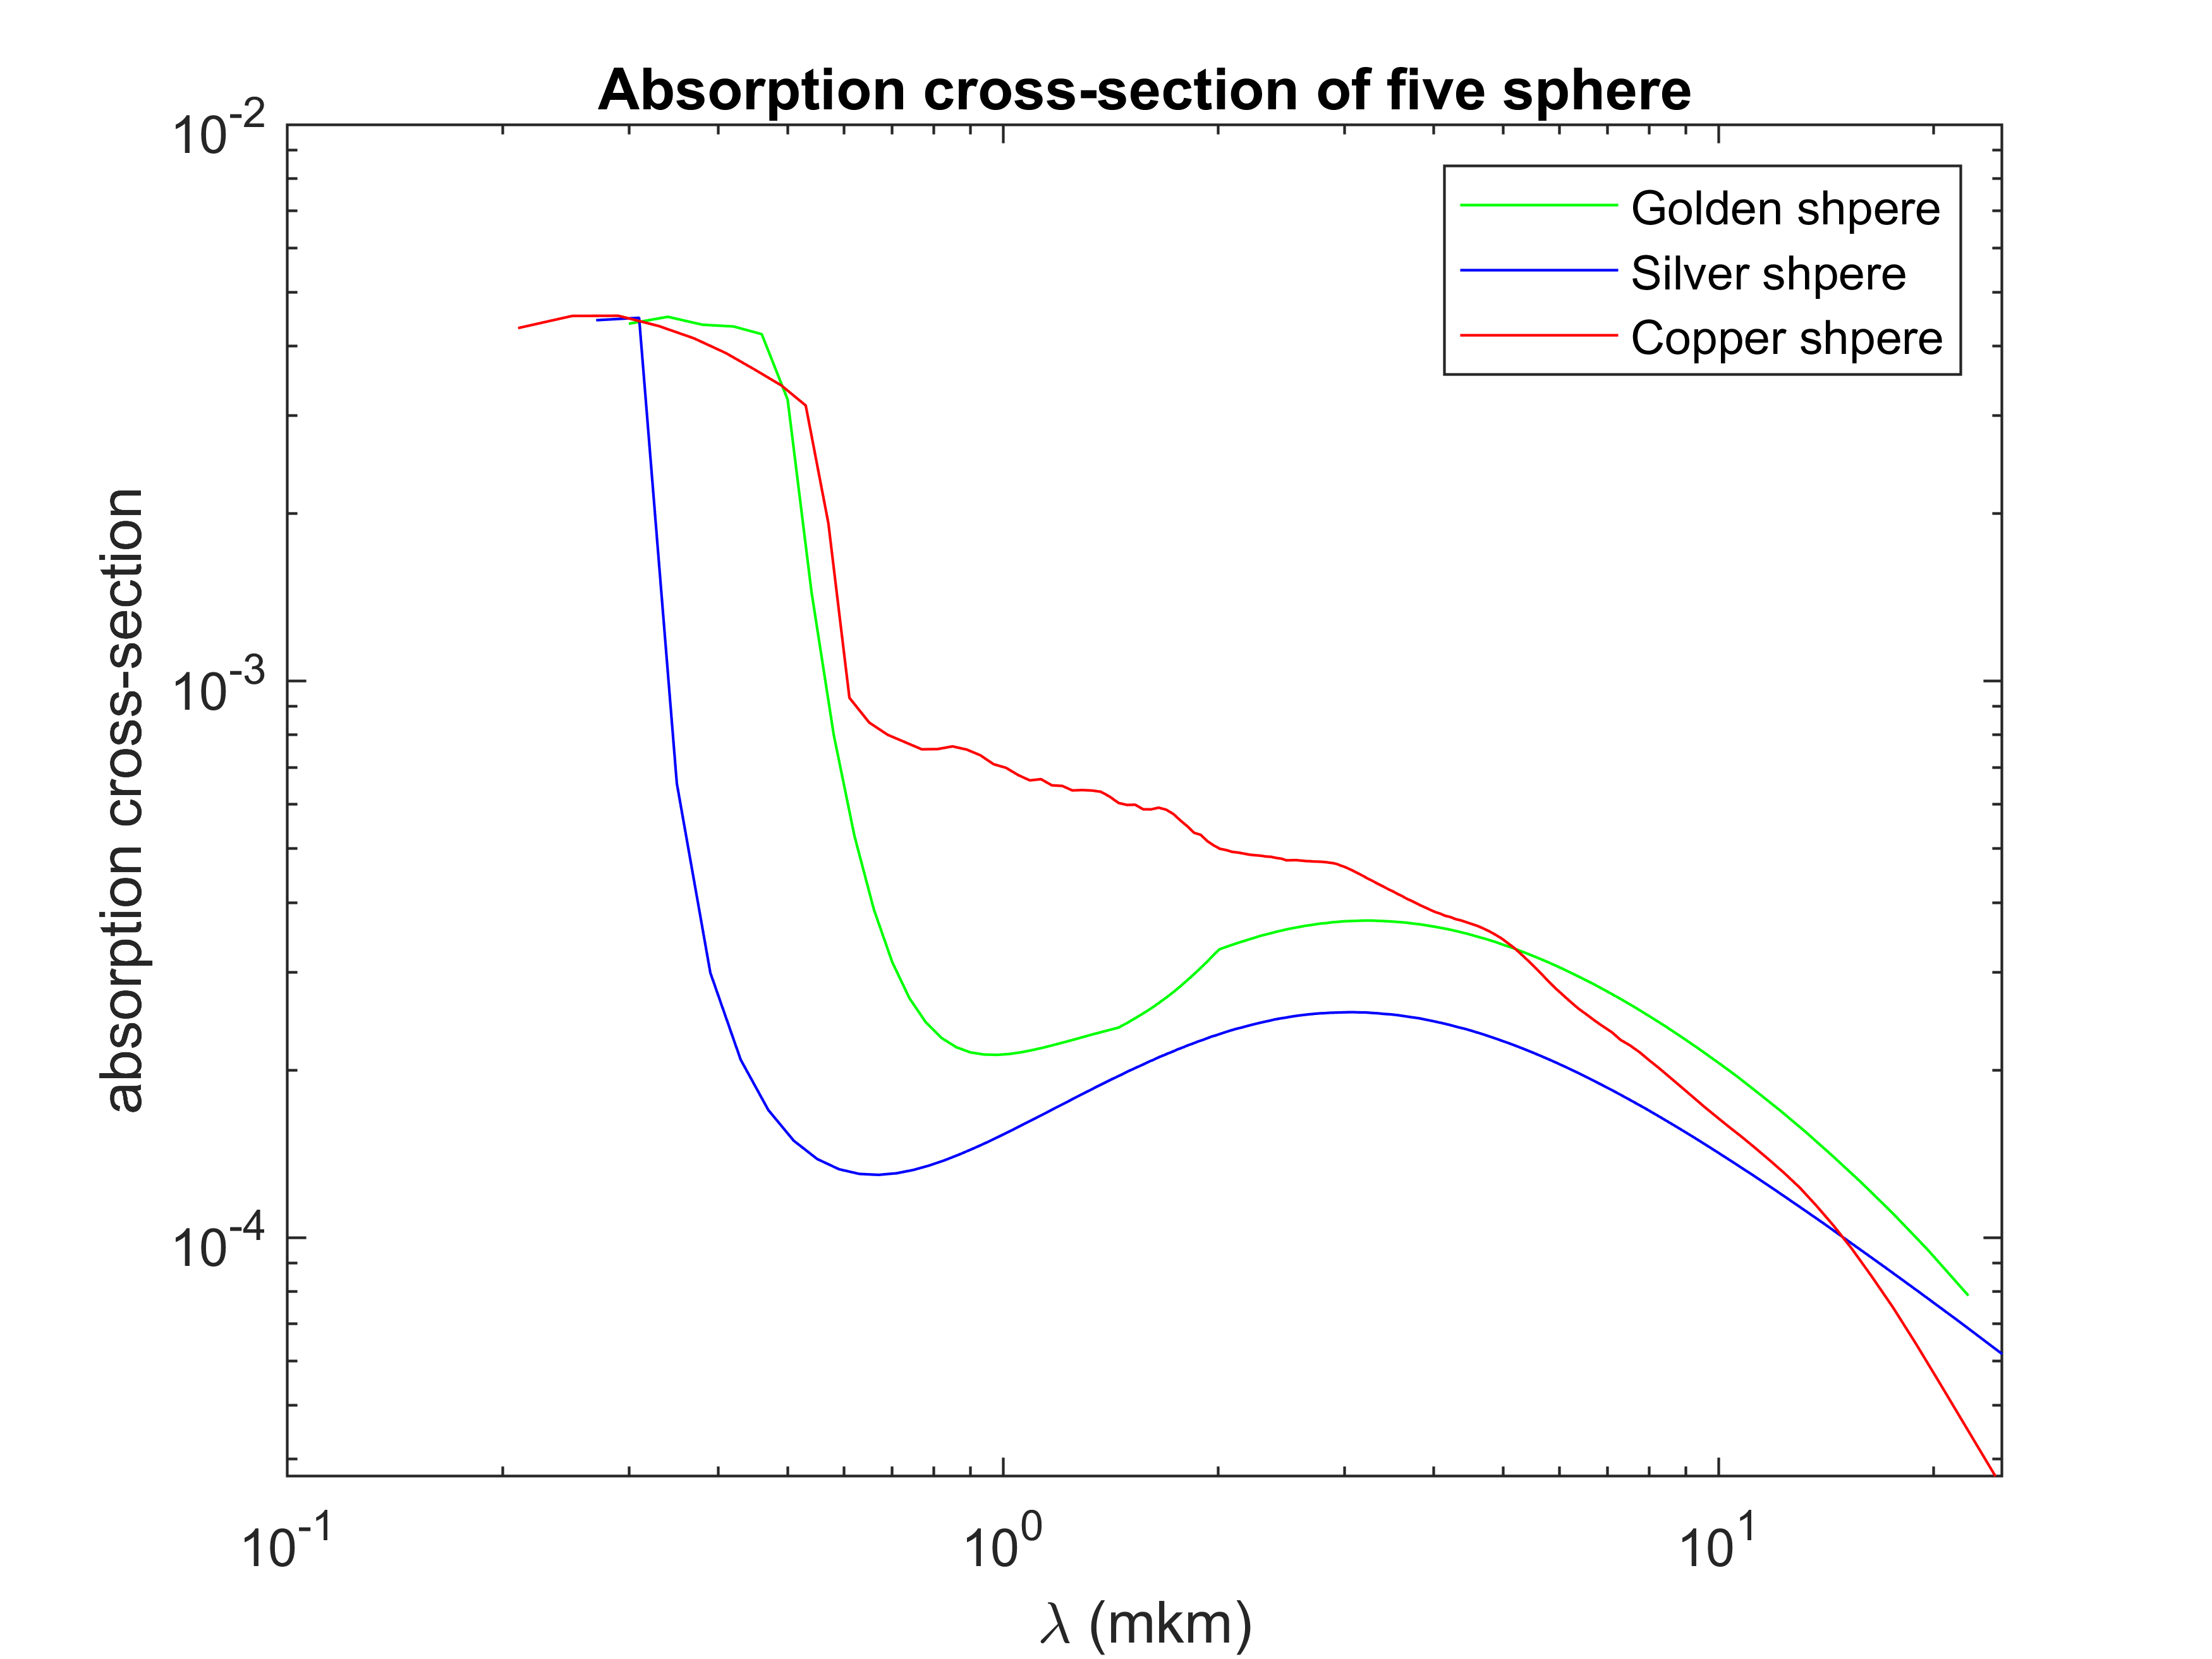
\includegraphics[width=0.8\linewidth]{absorpForFIVE}
	\caption{Сечение поглощения для пяти шаров в разных средах}
	\label{fig:absorpForFIVE}
\end{figure} 
\begin{figure}[h!]
	\centering
	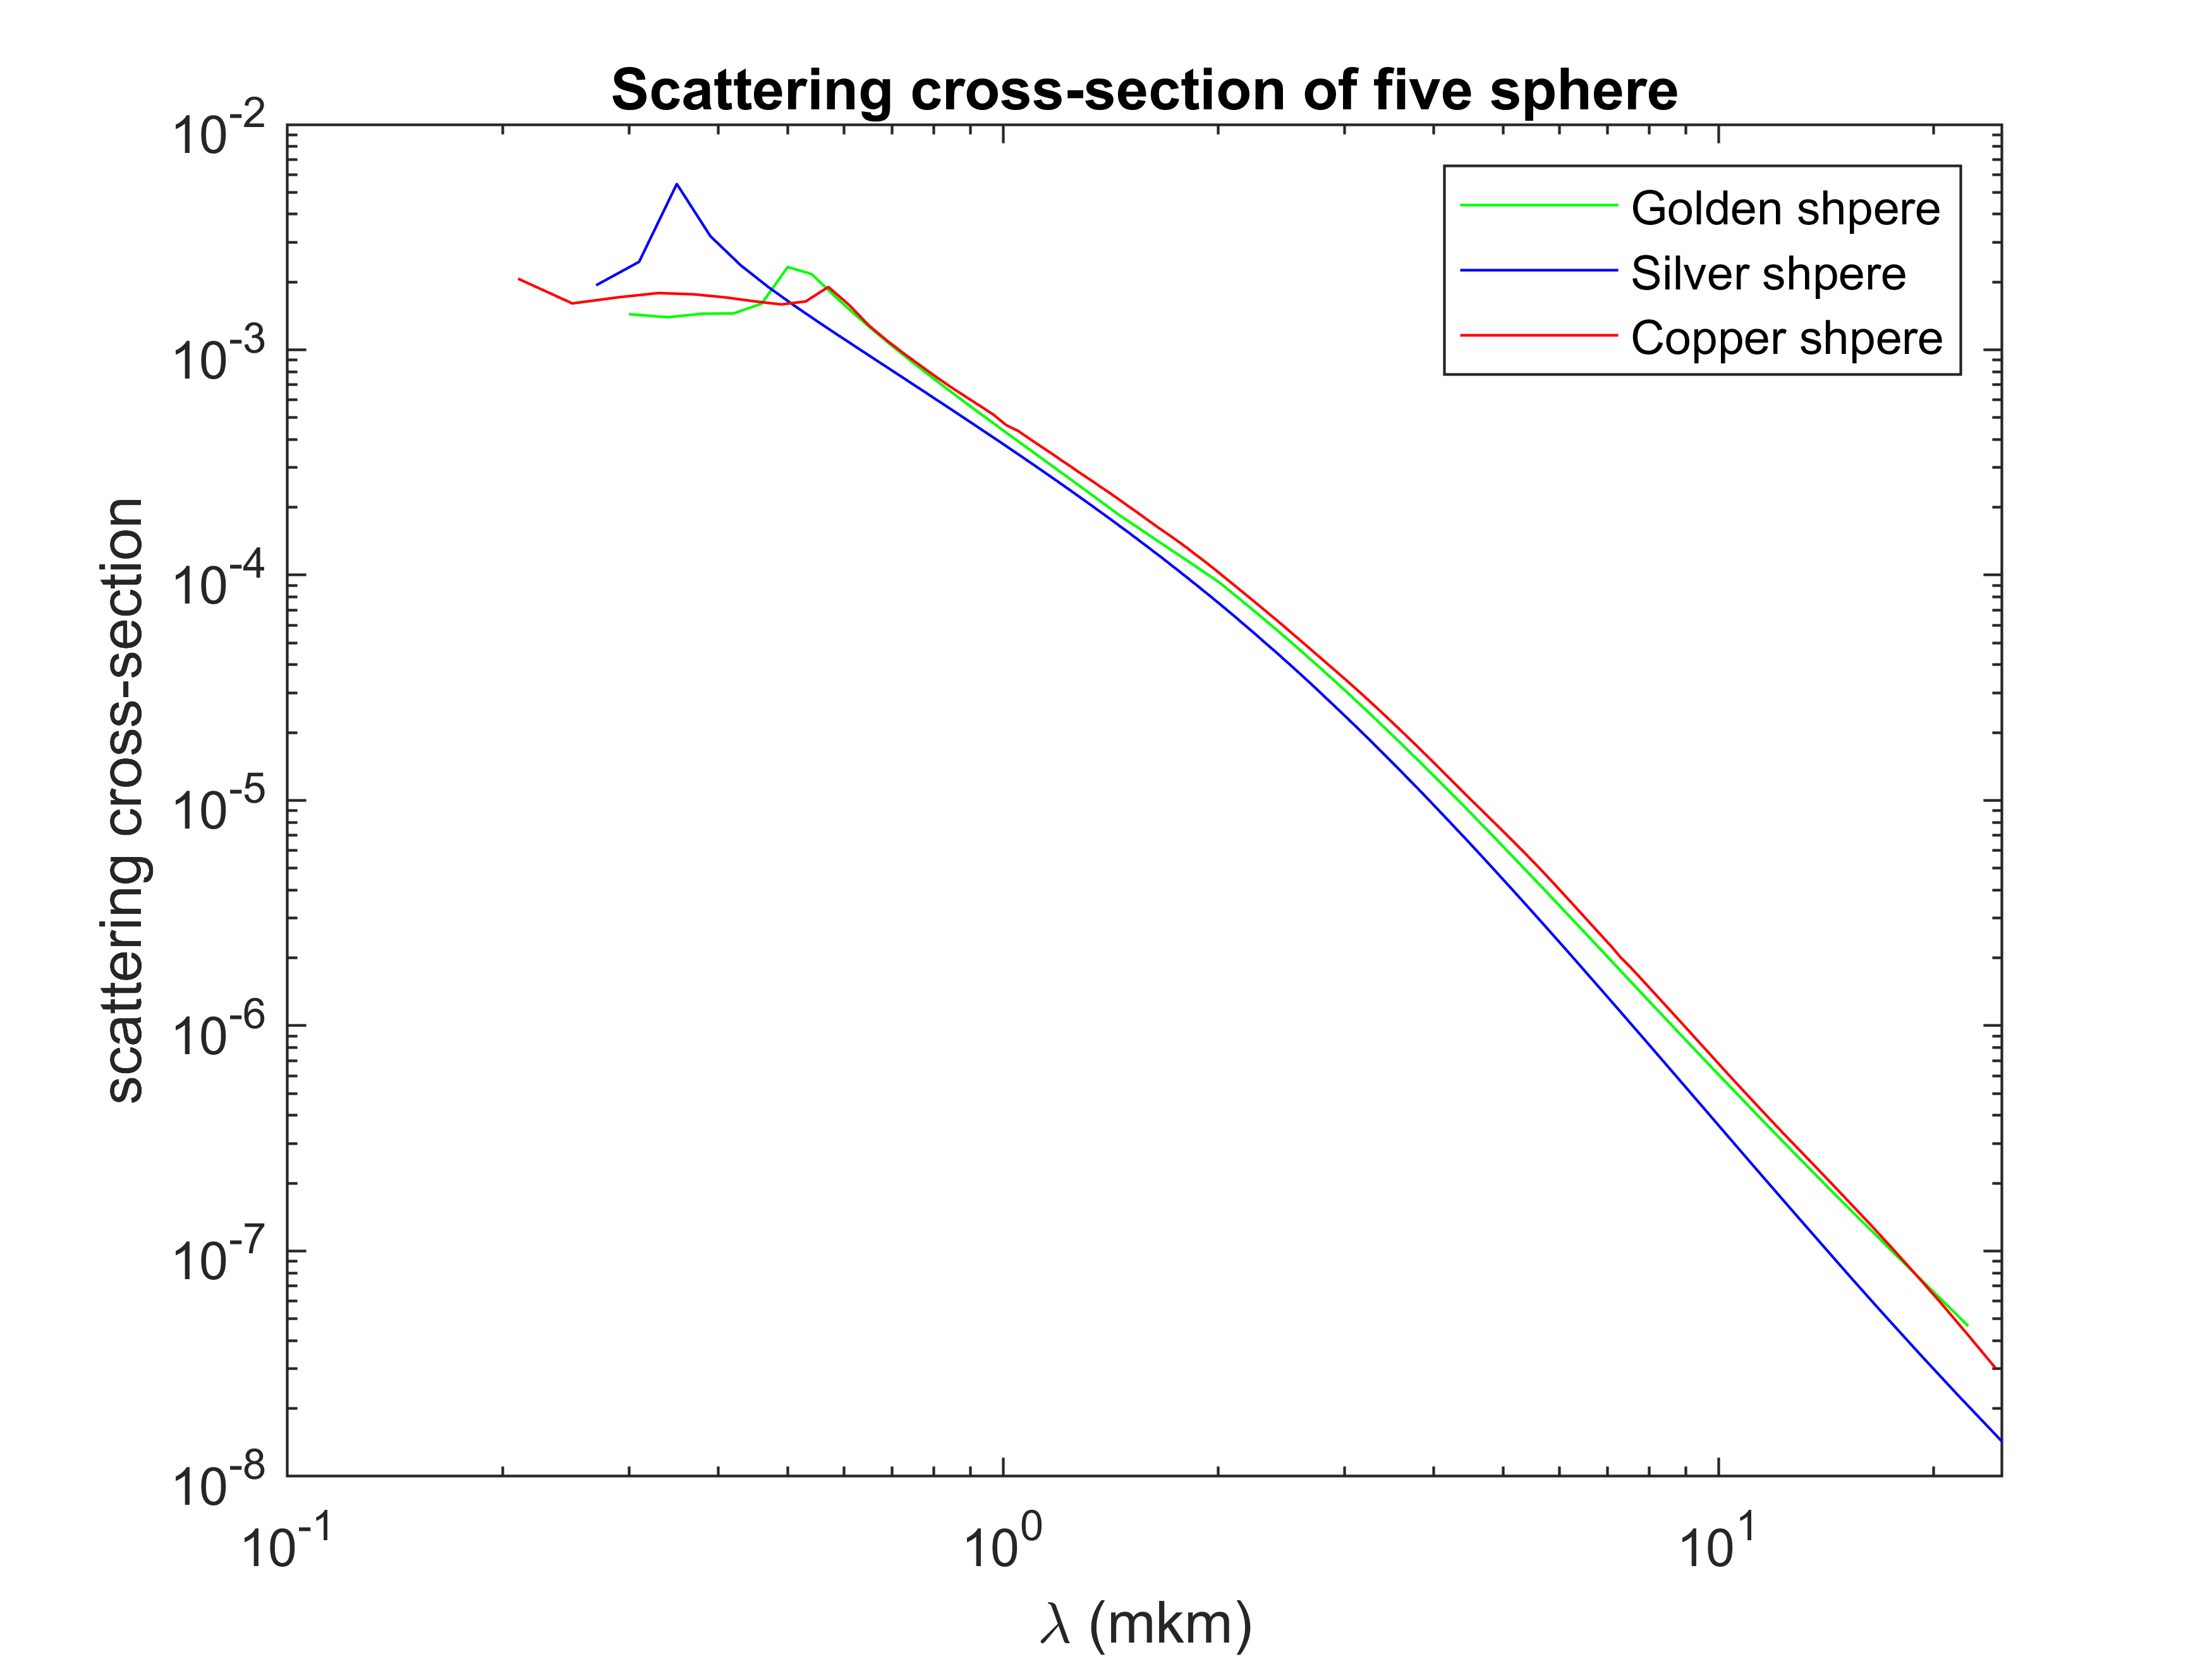
\includegraphics[width=0.8\linewidth]{scatForFIVE}
	\caption{Сечение рассеяния для пяти шаров в разных средах}
	\label{fig:scatForFIVE}
\end{figure} 
\begin{figure}[h!]
	\centering
	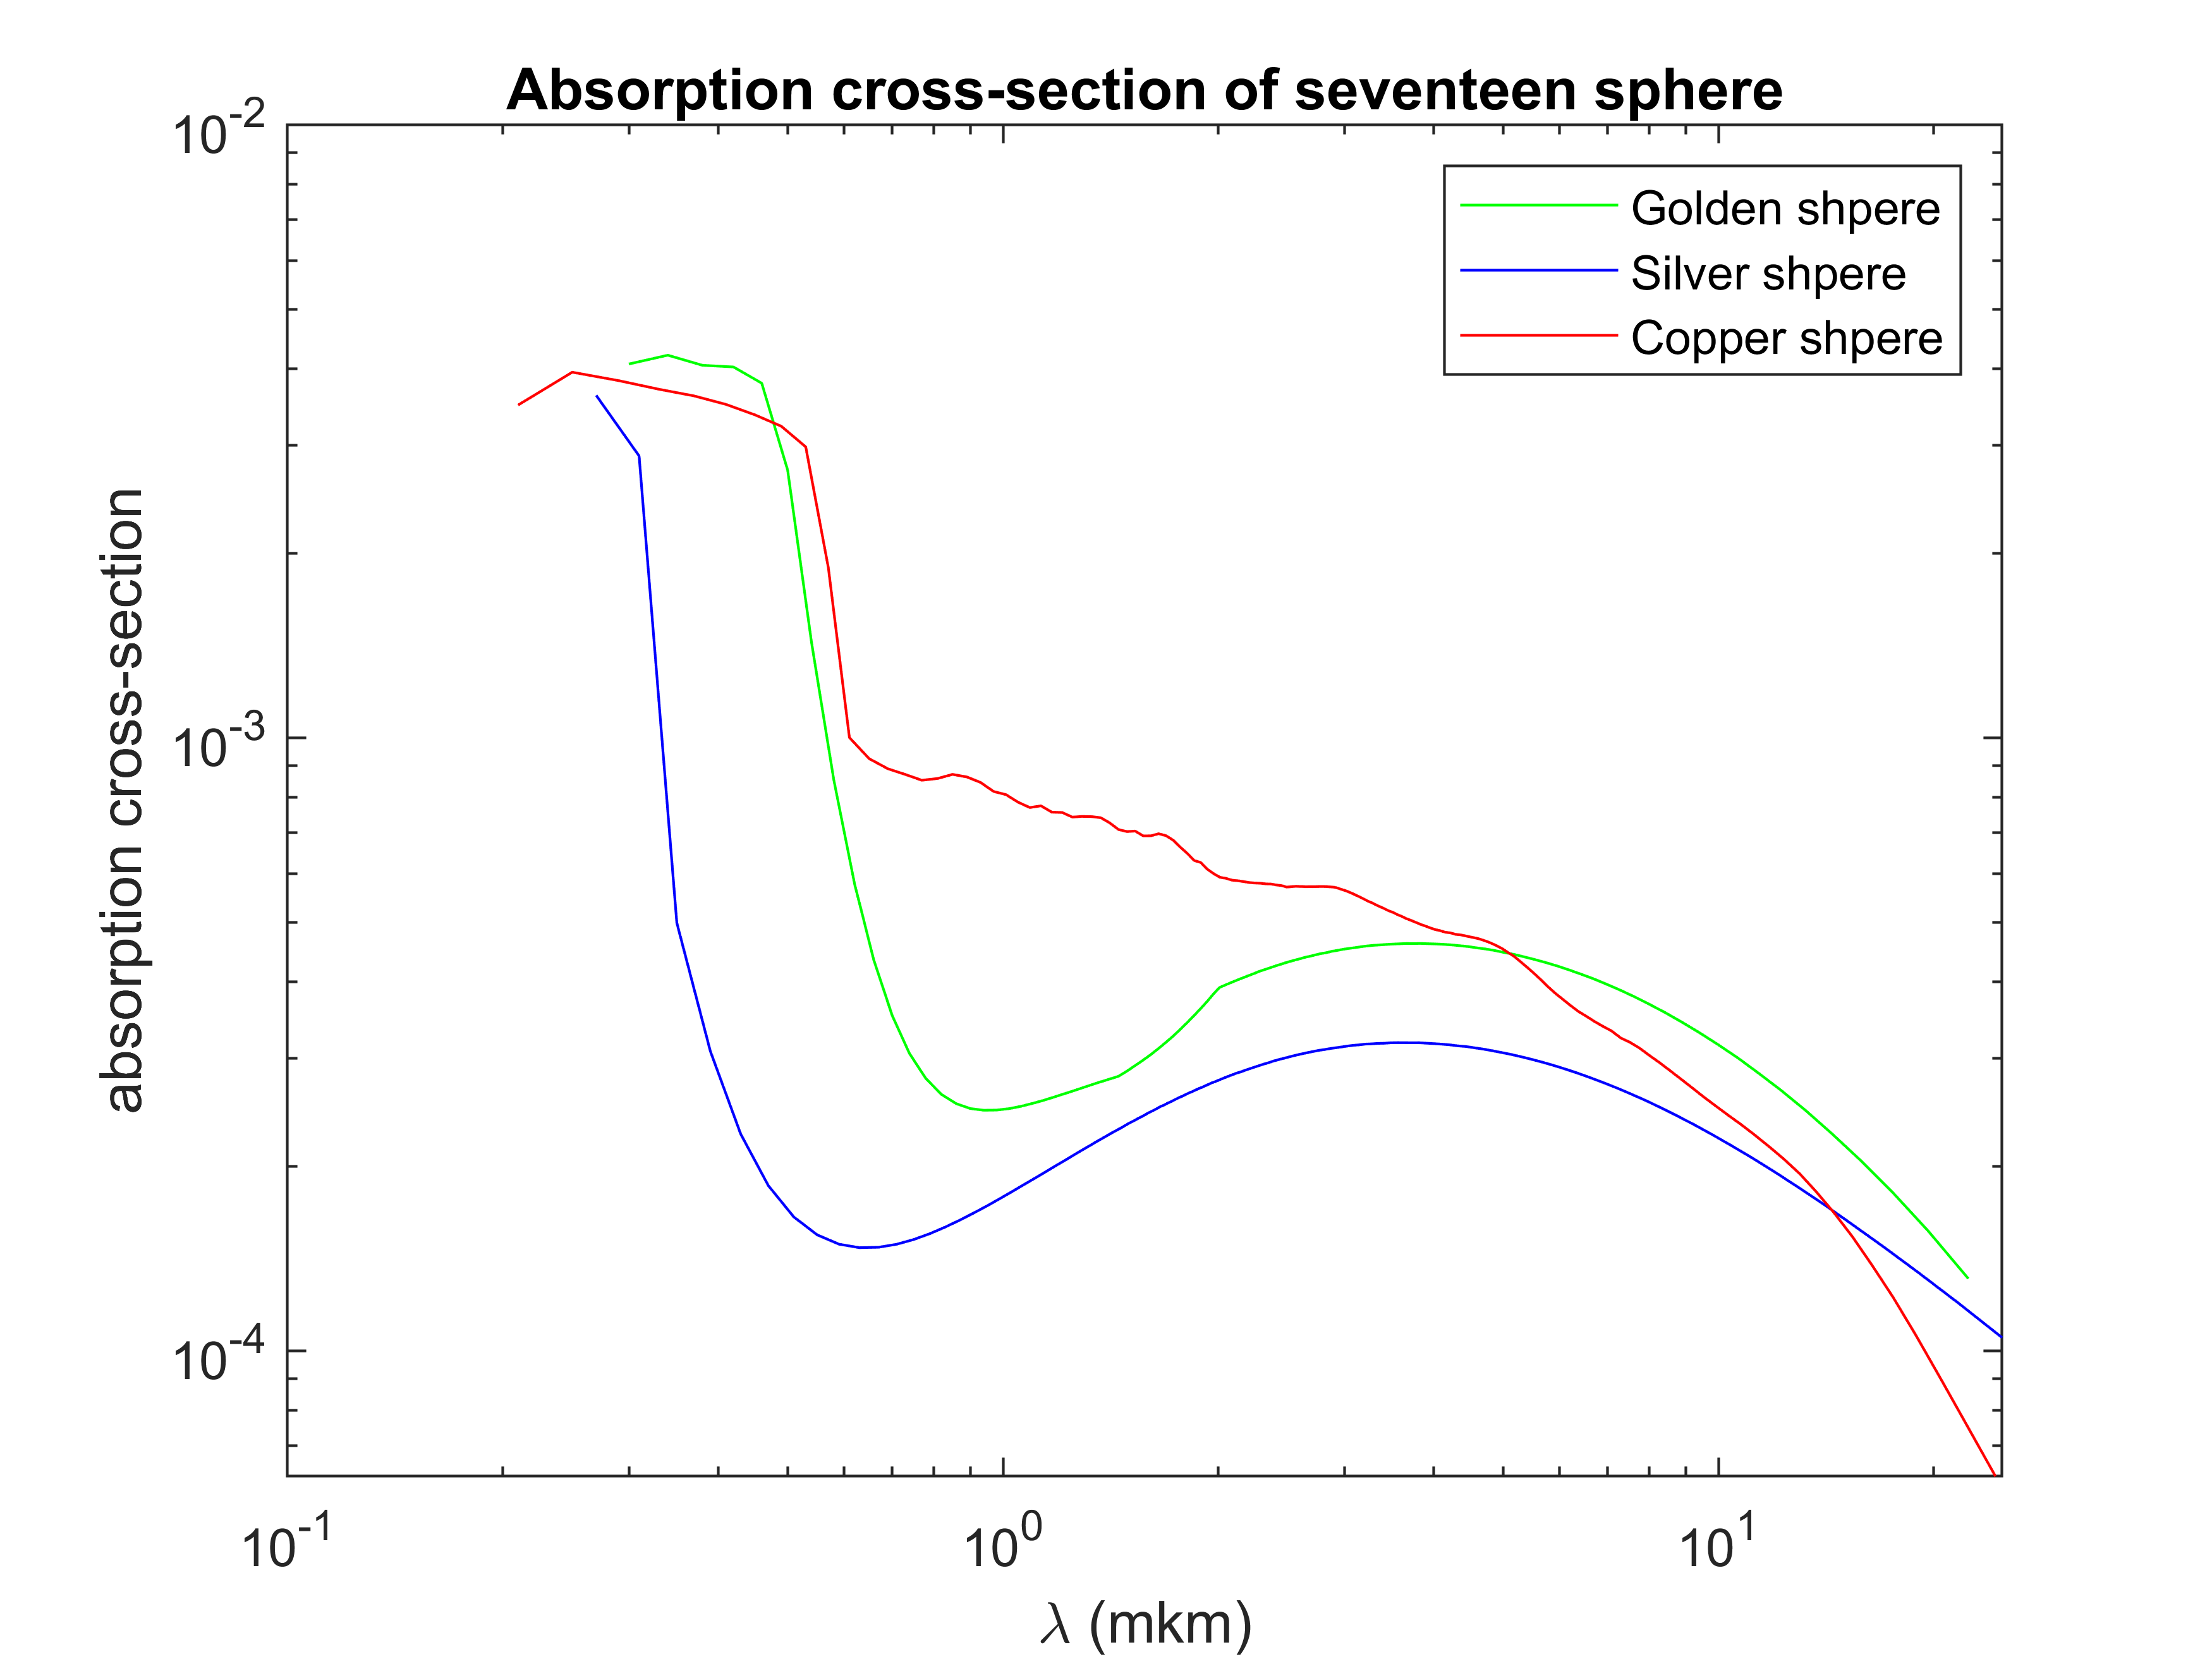
\includegraphics[width=0.8\linewidth]{absorpForSEVENTEEN}
	\caption{Сечение поглощения для семнадцати шаров в разных средах}
	\label{fig:absorpForSEVENTEEN}
\end{figure}
\begin{figure}[h!]
	\centering
	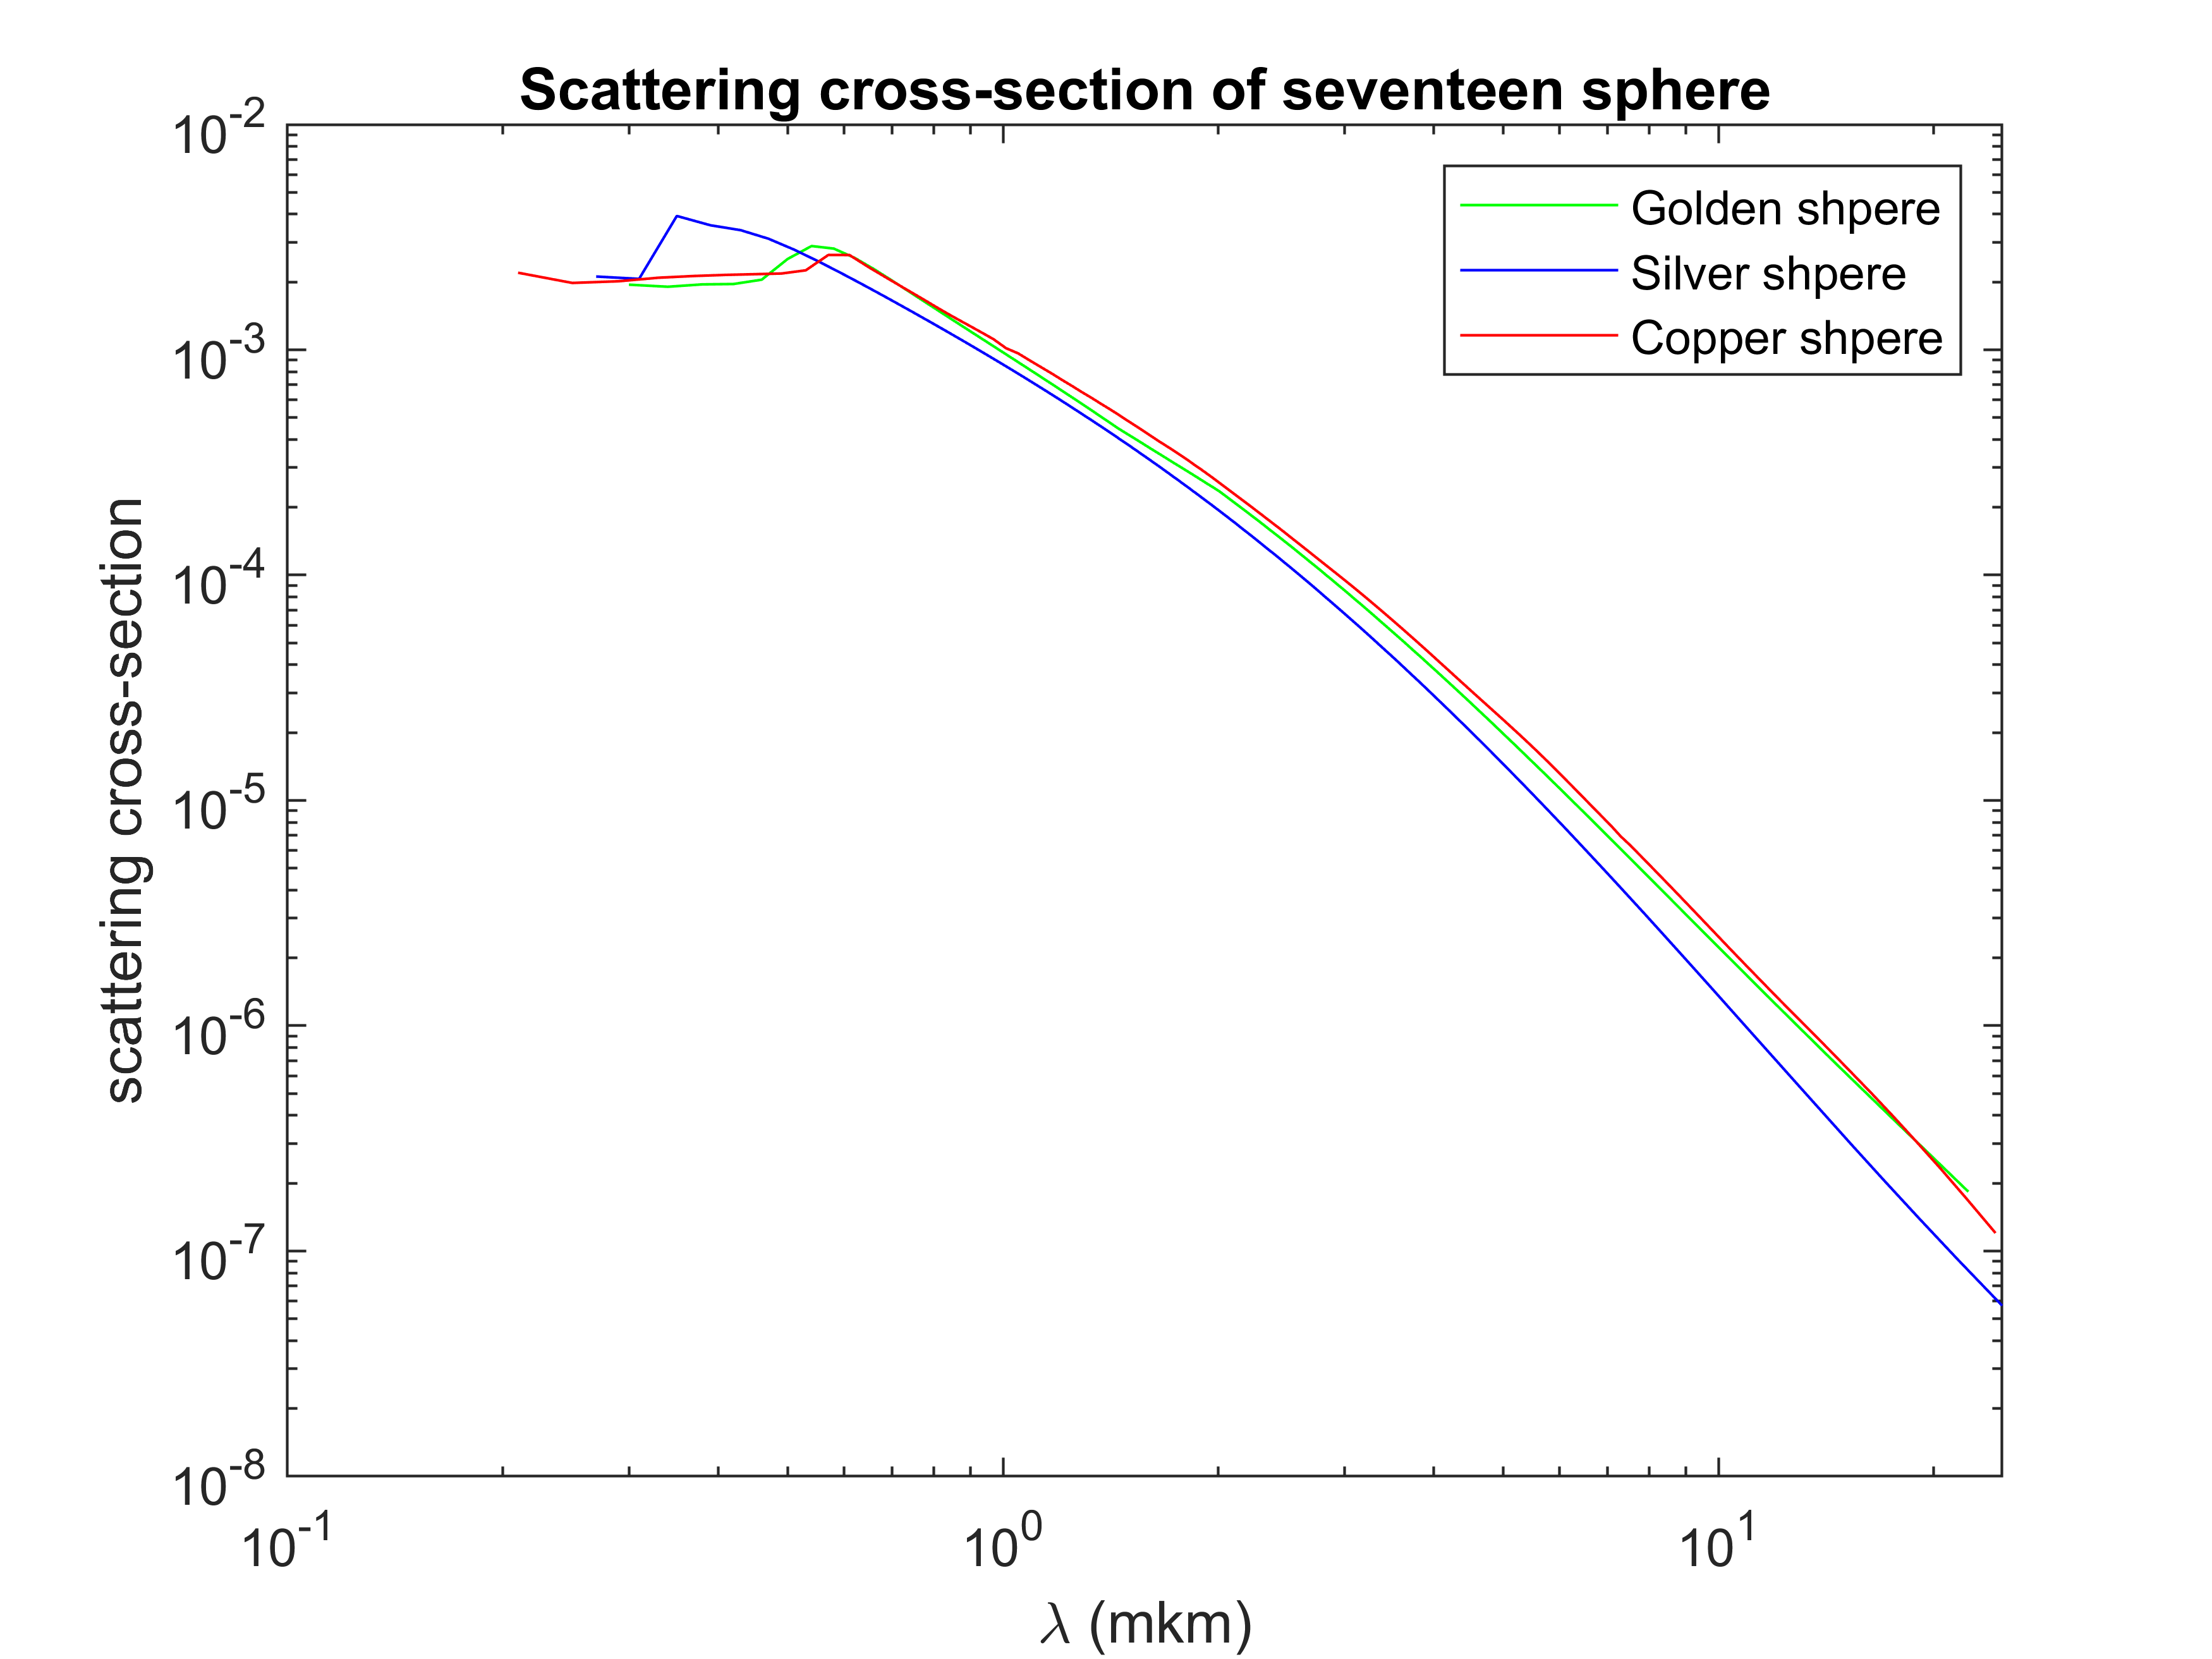
\includegraphics[width=0.8\linewidth]{scatForSEVENTEEN}
	\caption{Сечение рассеяния для семнадцати шаров в разных средах}
	\label{fig:scatForSEVENTEEN}
\end{figure} 

\begin{figure}[h!]
	\centering
	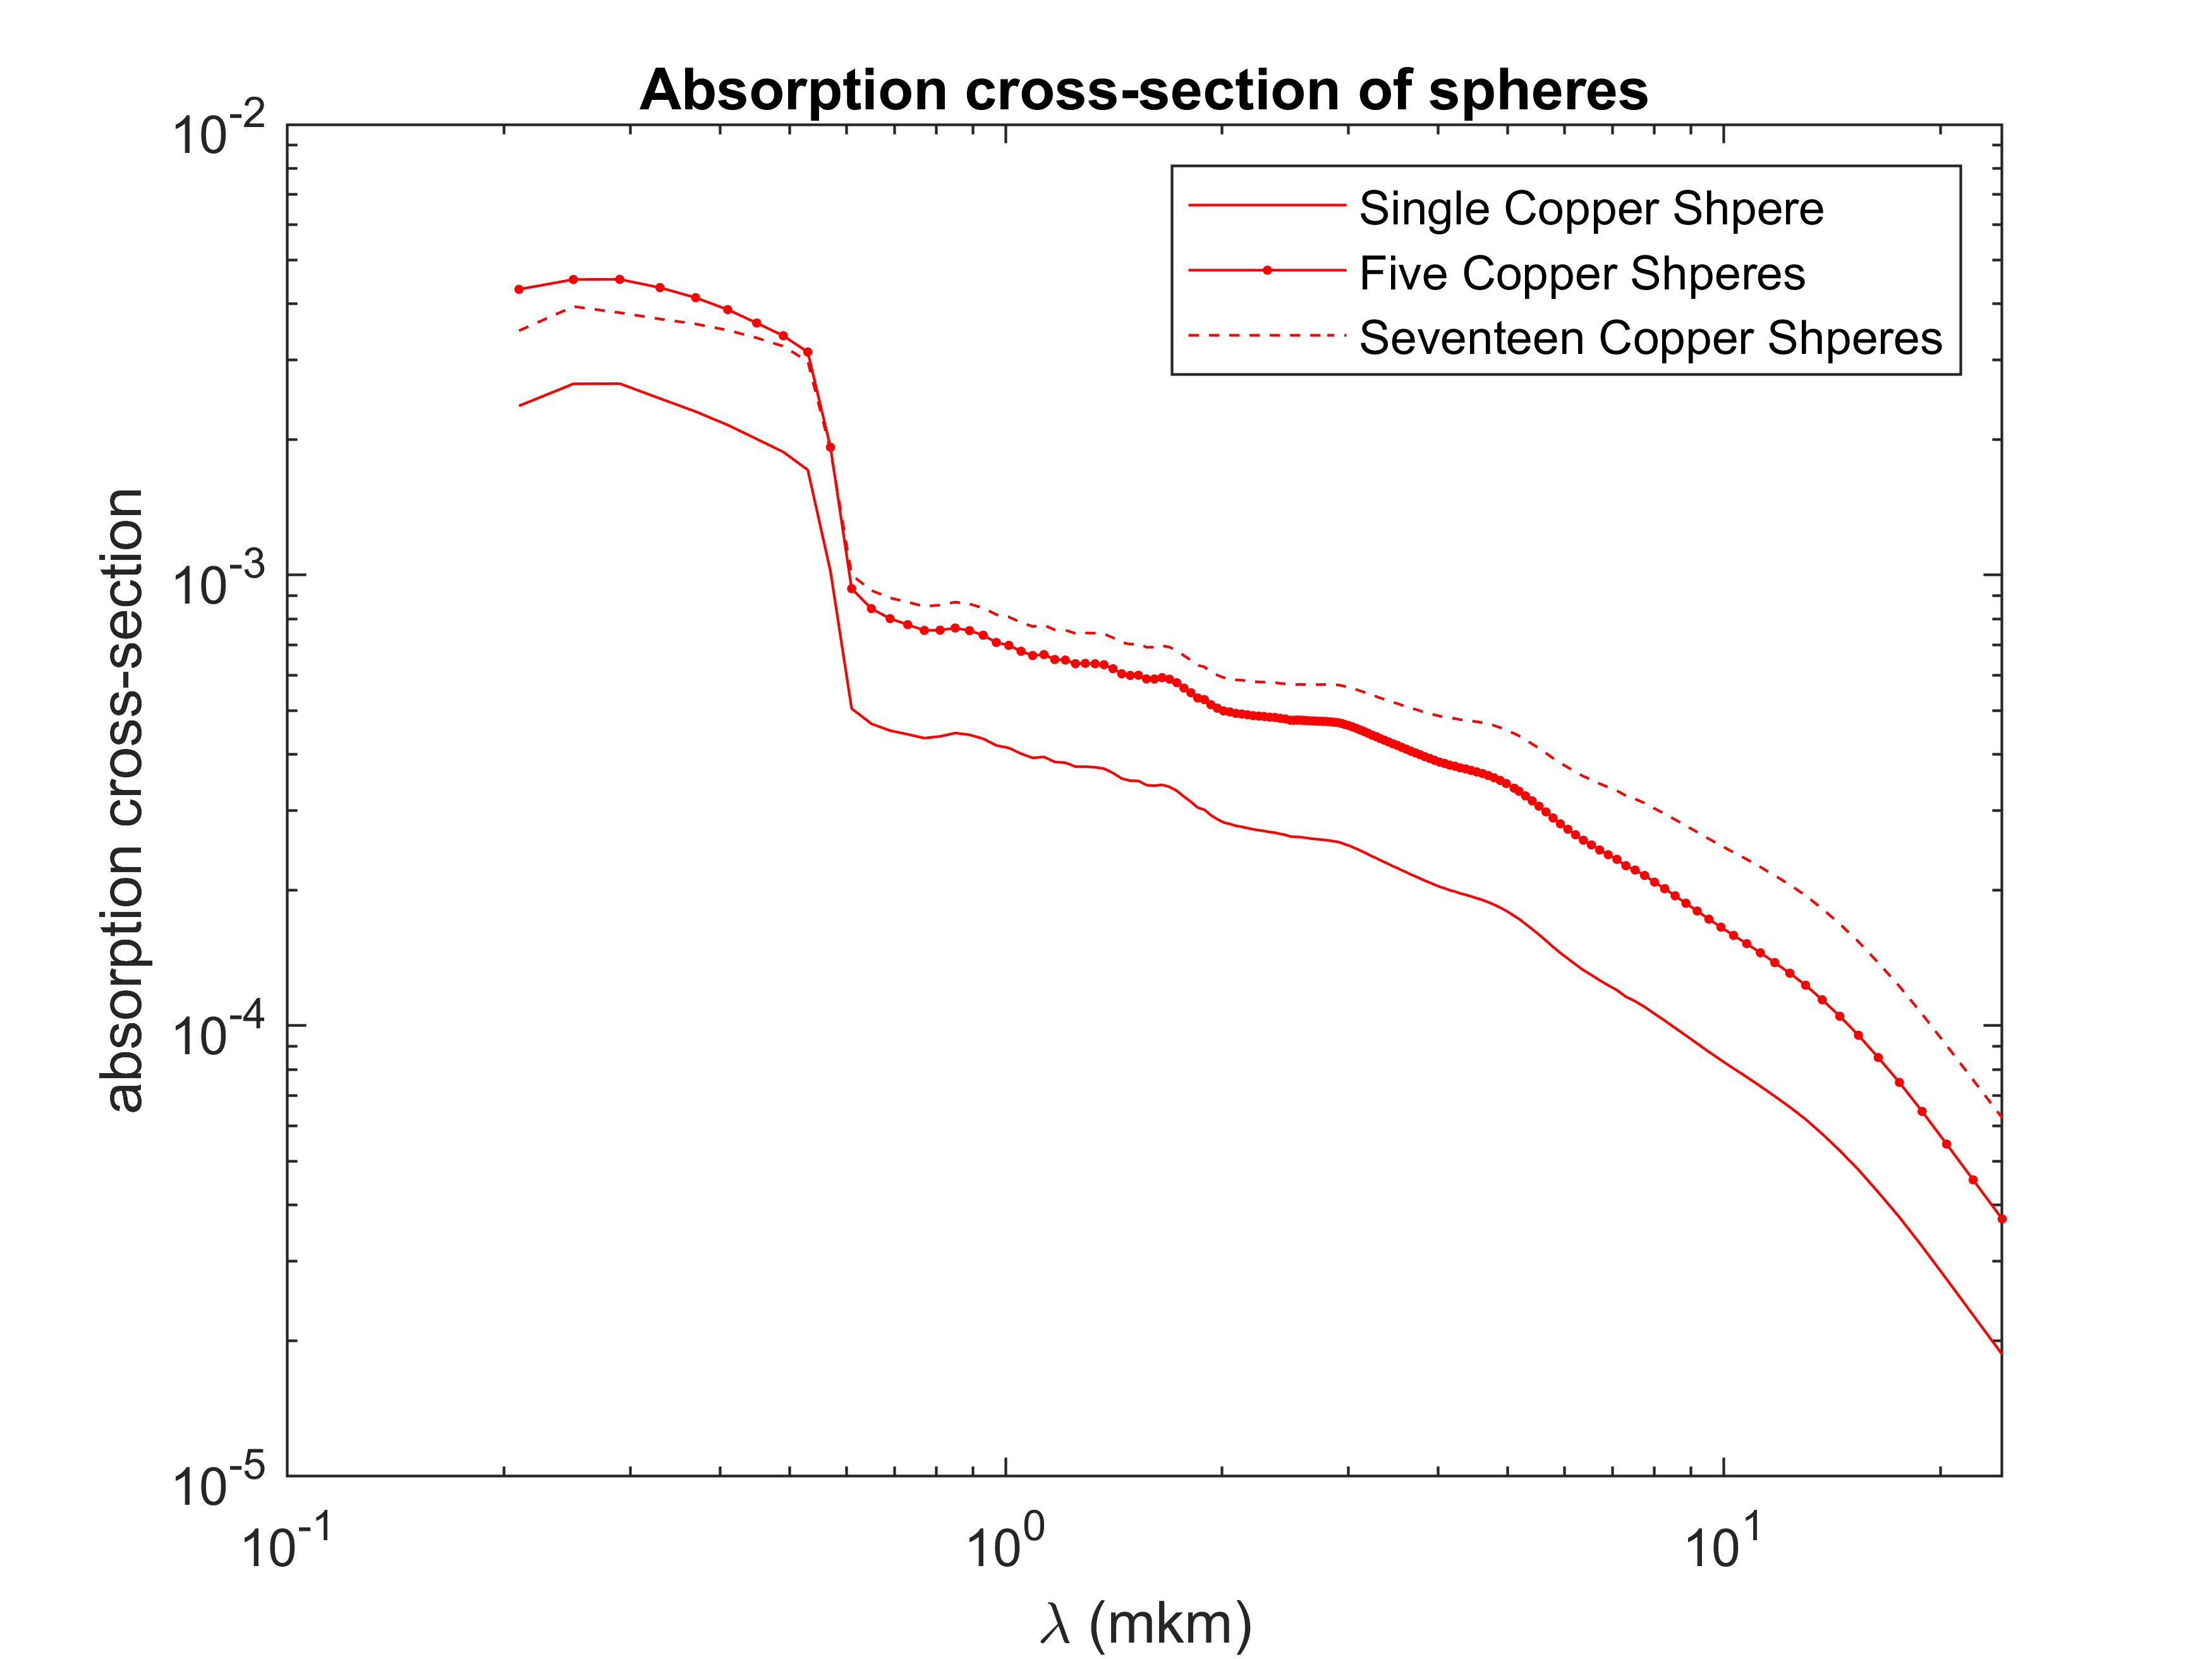
\includegraphics[width=0.8\linewidth]{absorpForCopper}
	\caption{Сечение поглощения для медных шаров}
	\label{fig:absorpForCopper}
\end{figure}
\begin{figure}[h!]
	\centering
	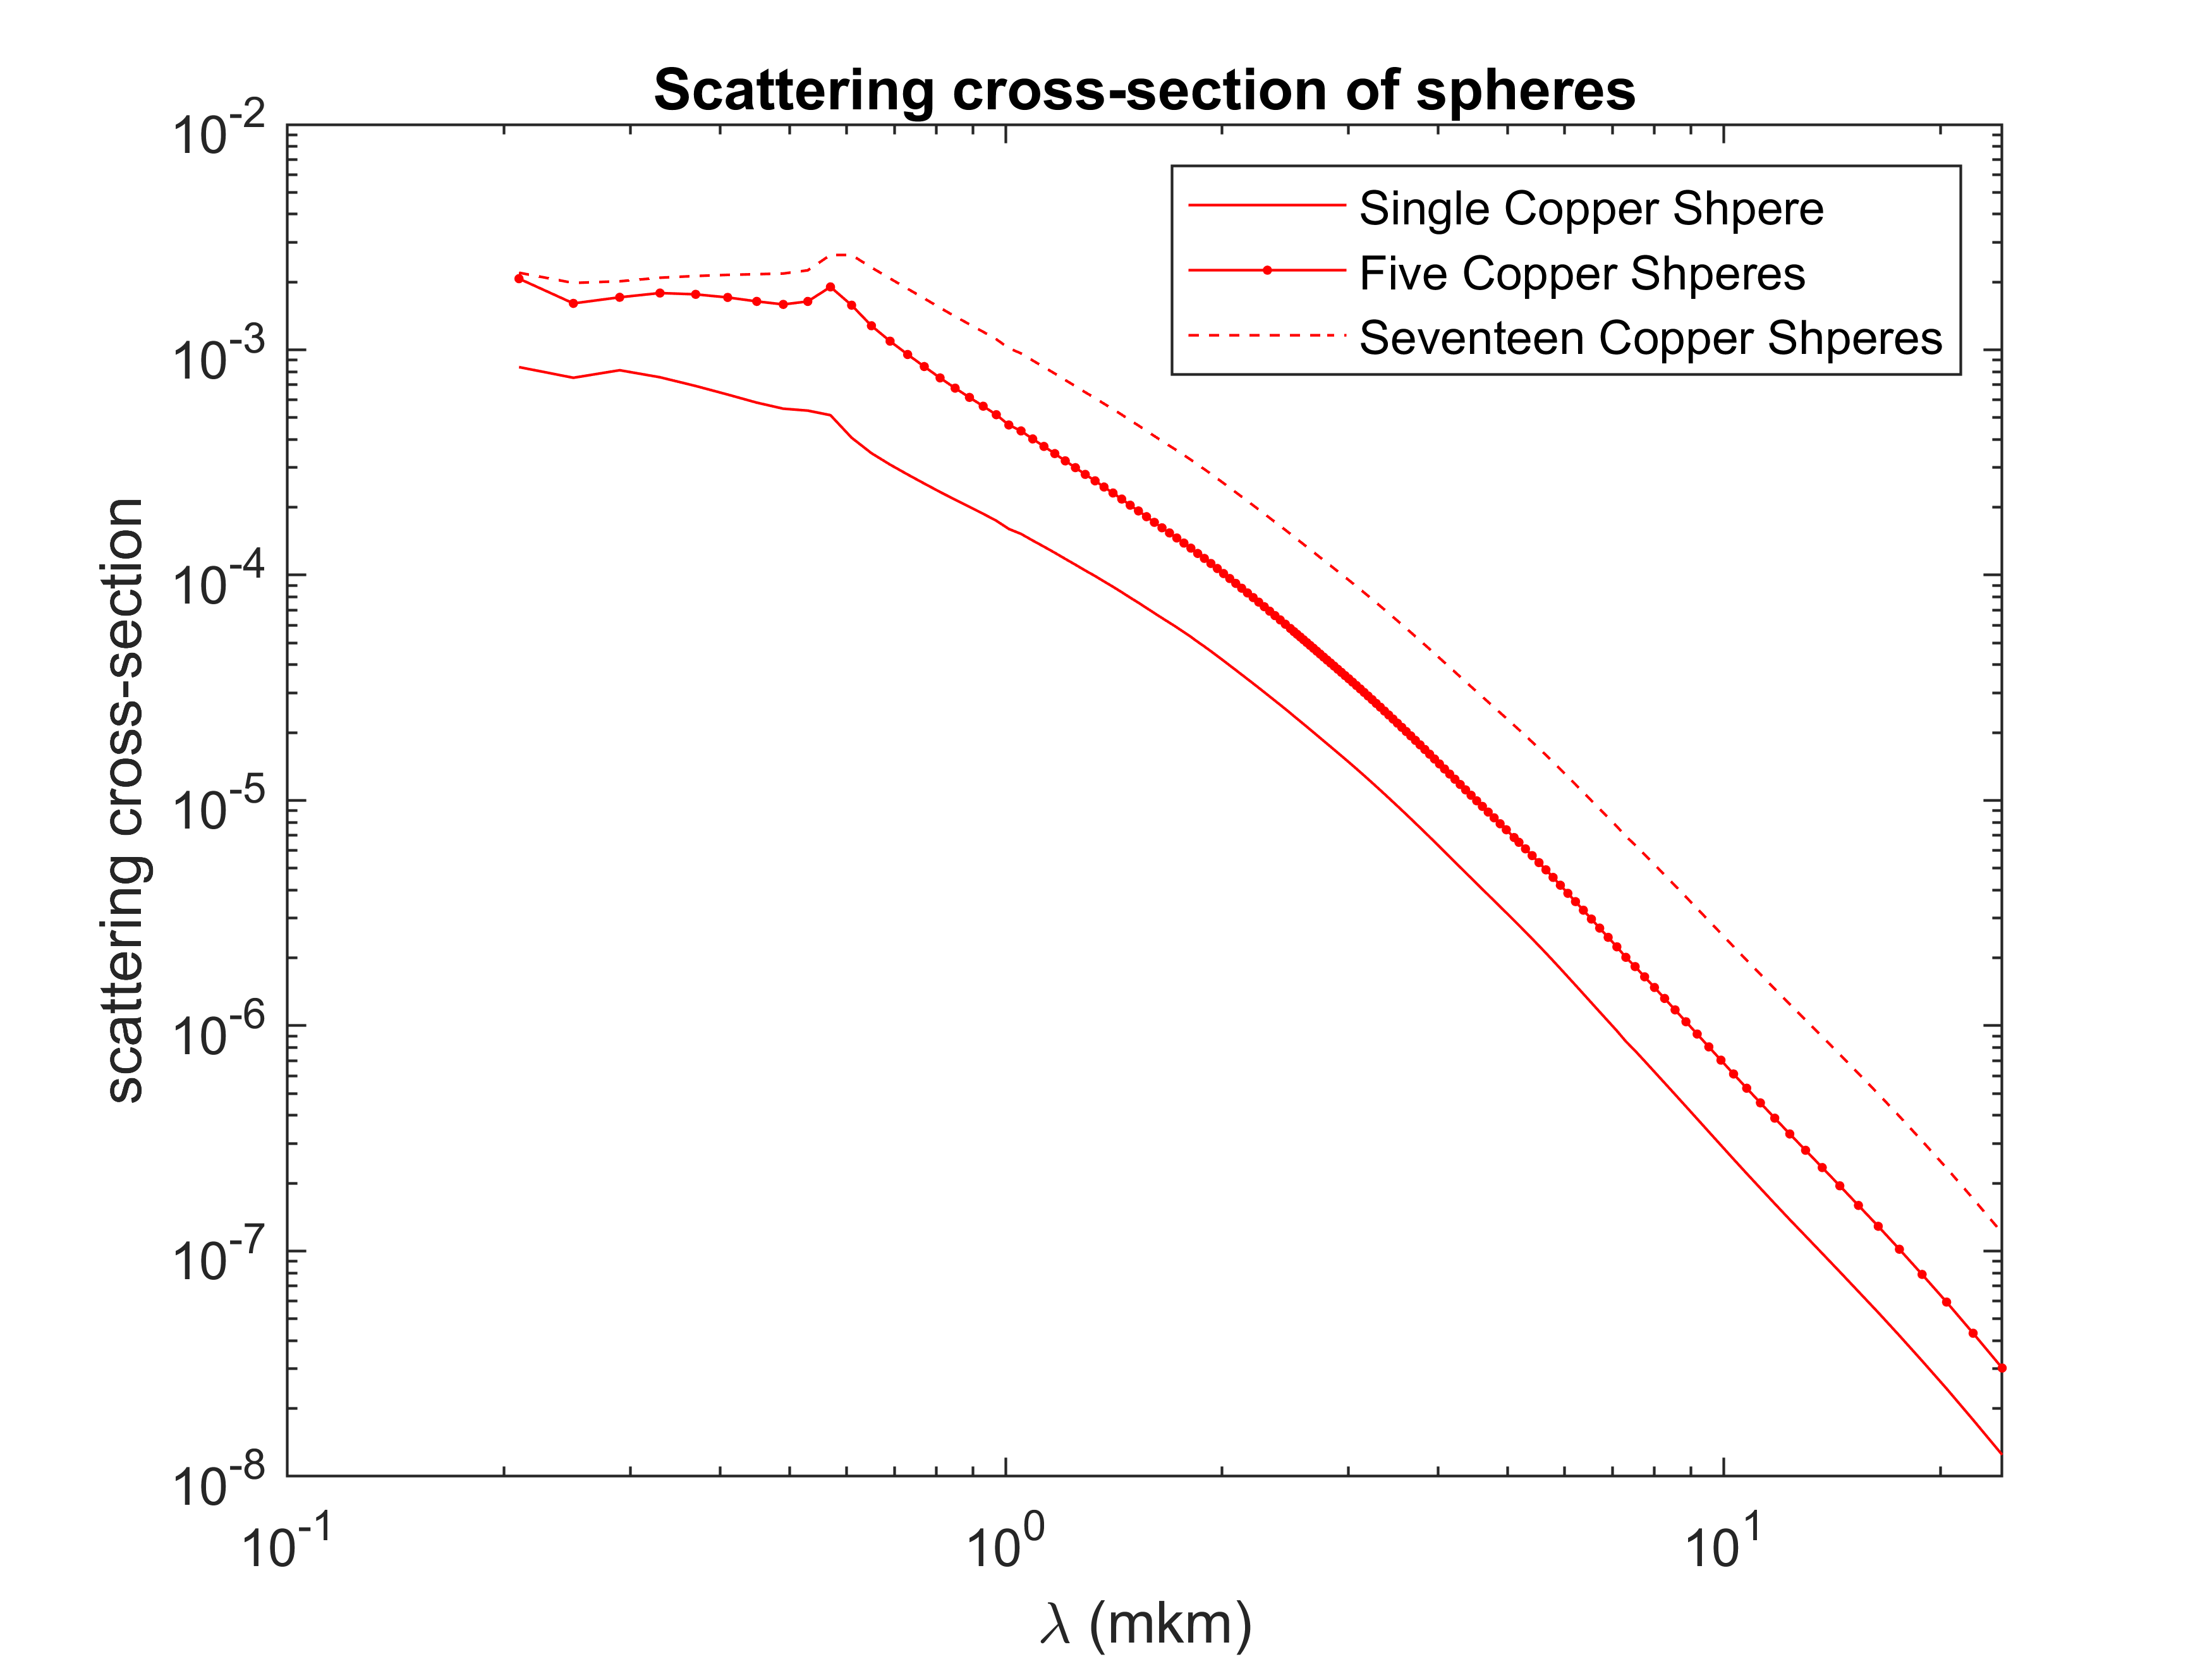
\includegraphics[width=0.8\linewidth]{scatForCopper}
	\caption{Сечение рассеяния для медных шаров}
	\label{fig:scatForCopper}
\end{figure} 
\begin{figure}[h!]
	\centering
	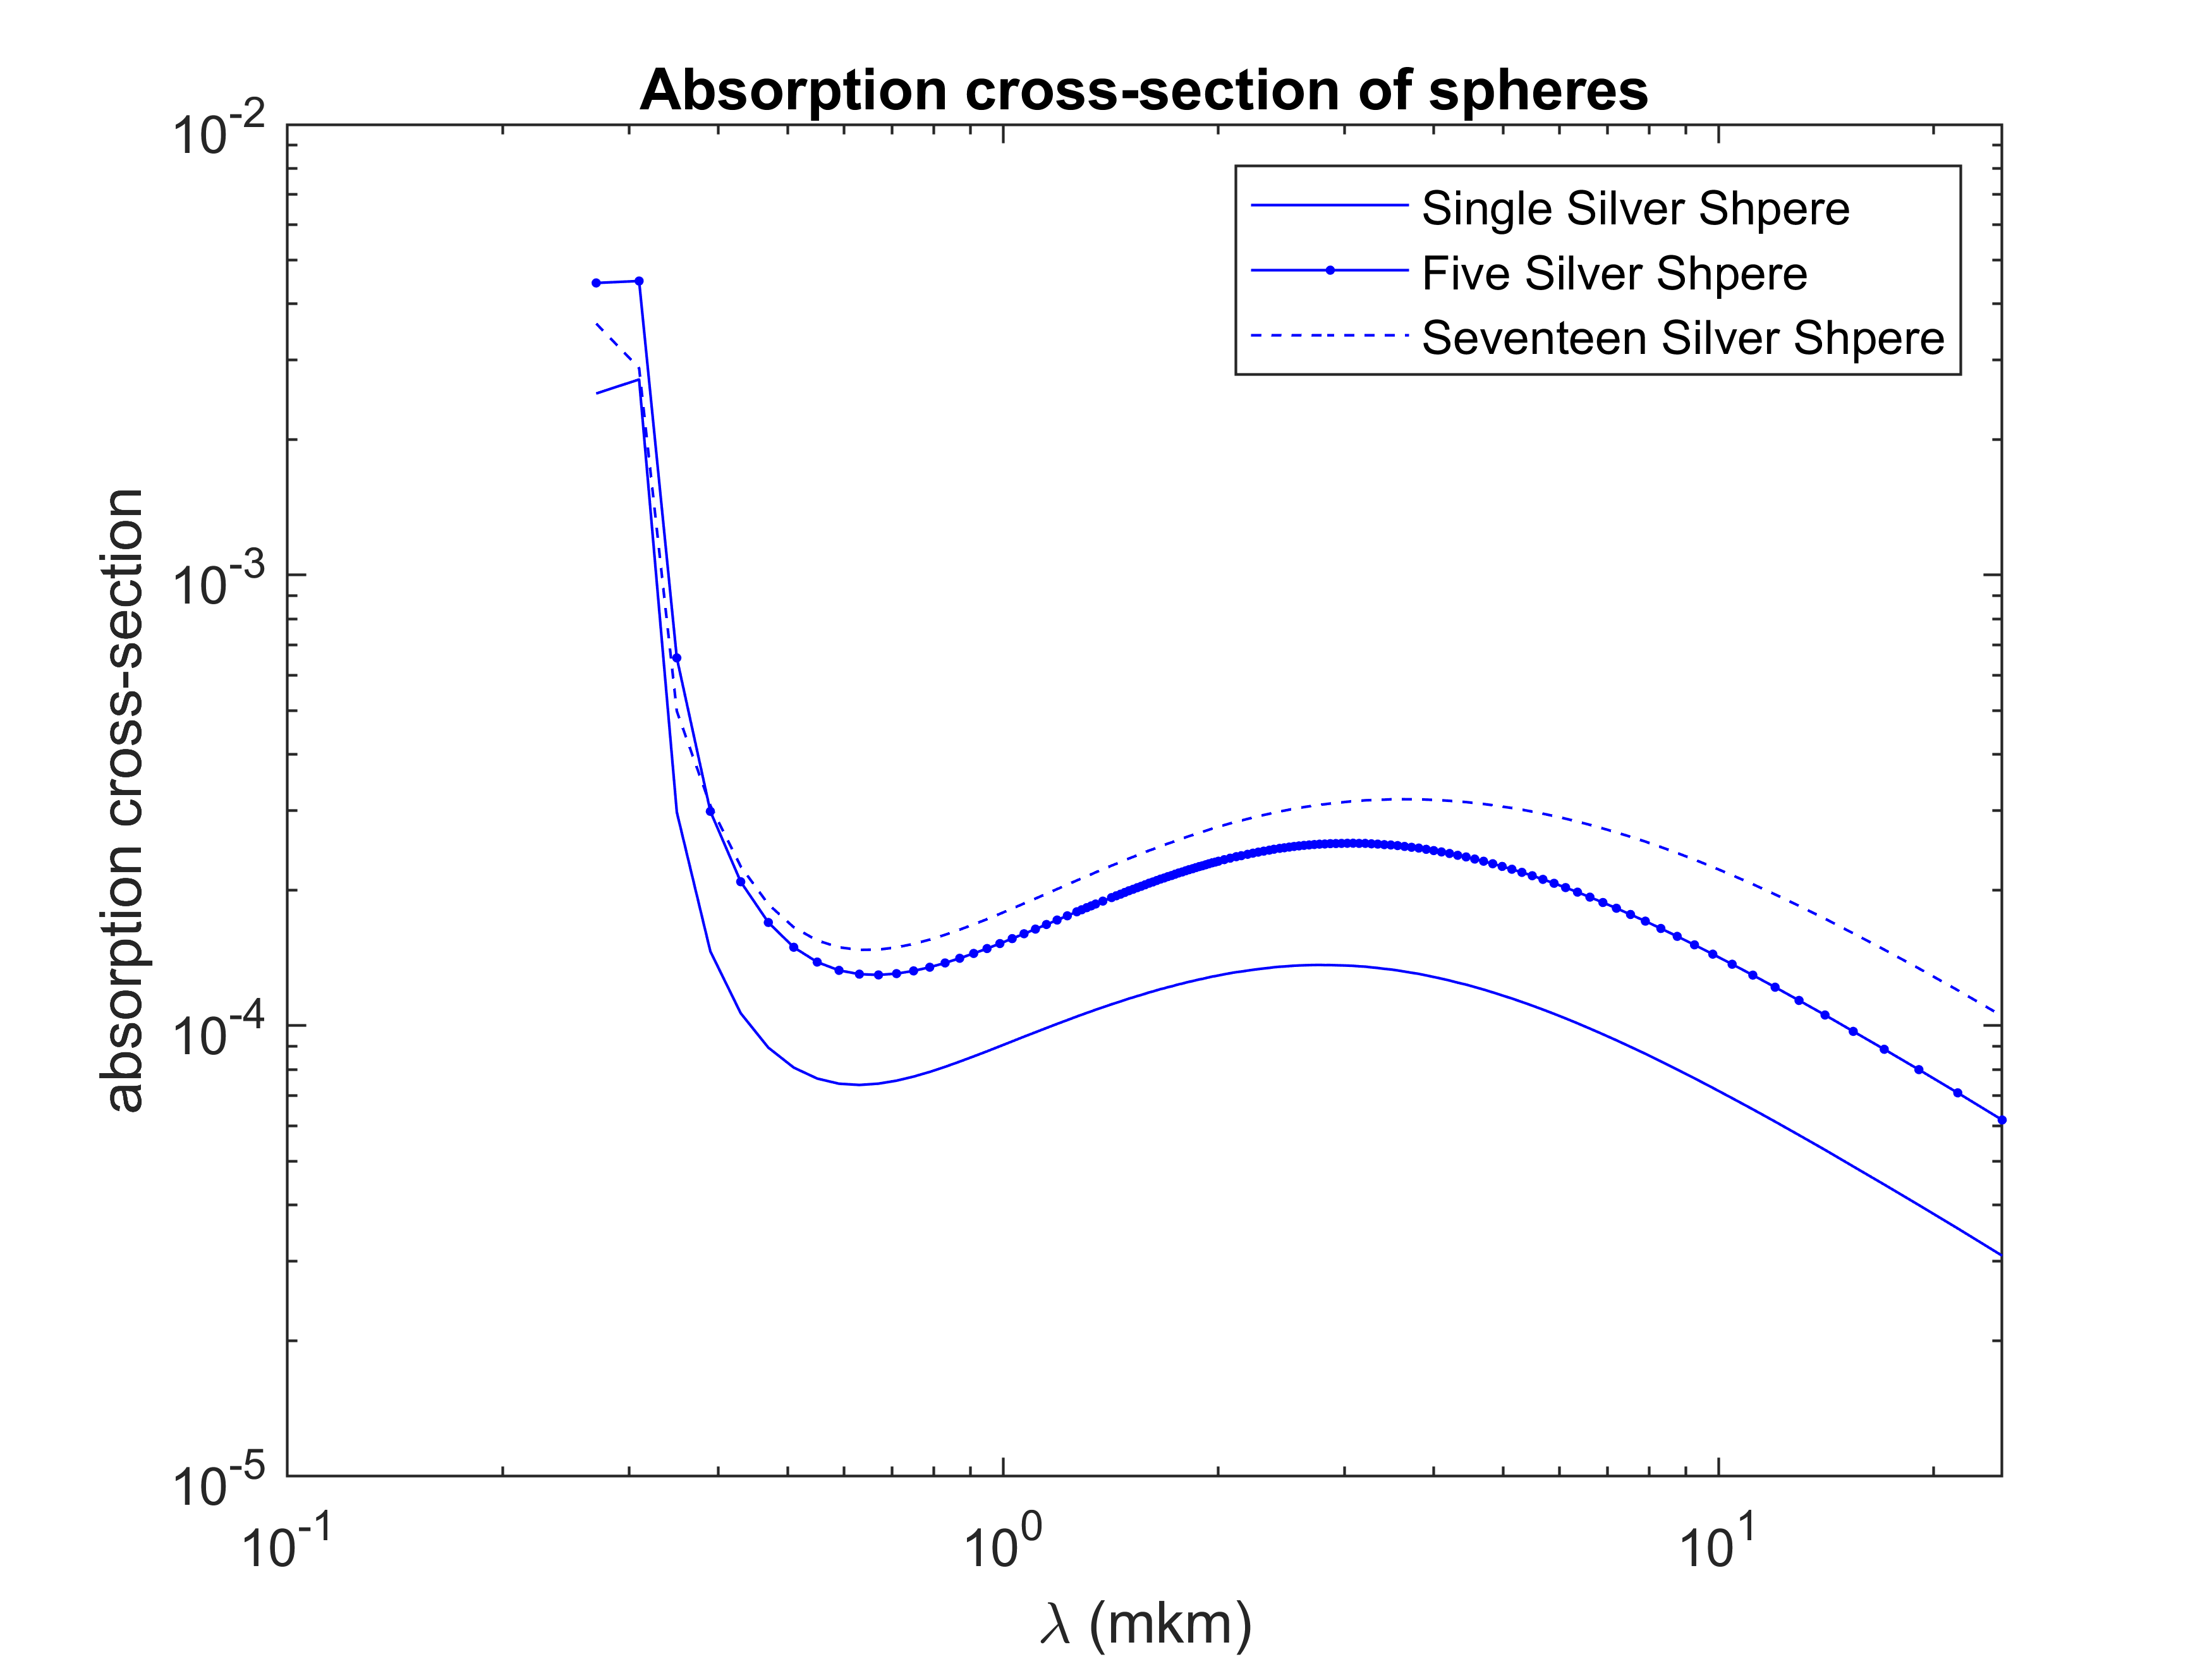
\includegraphics[width=0.8\linewidth]{absorpForSilver}
	\caption{Сечение поглощения для серебряных шаров}
	\label{fig:absorpForSilver}
\end{figure}
\begin{figure}[h!]
	\centering
	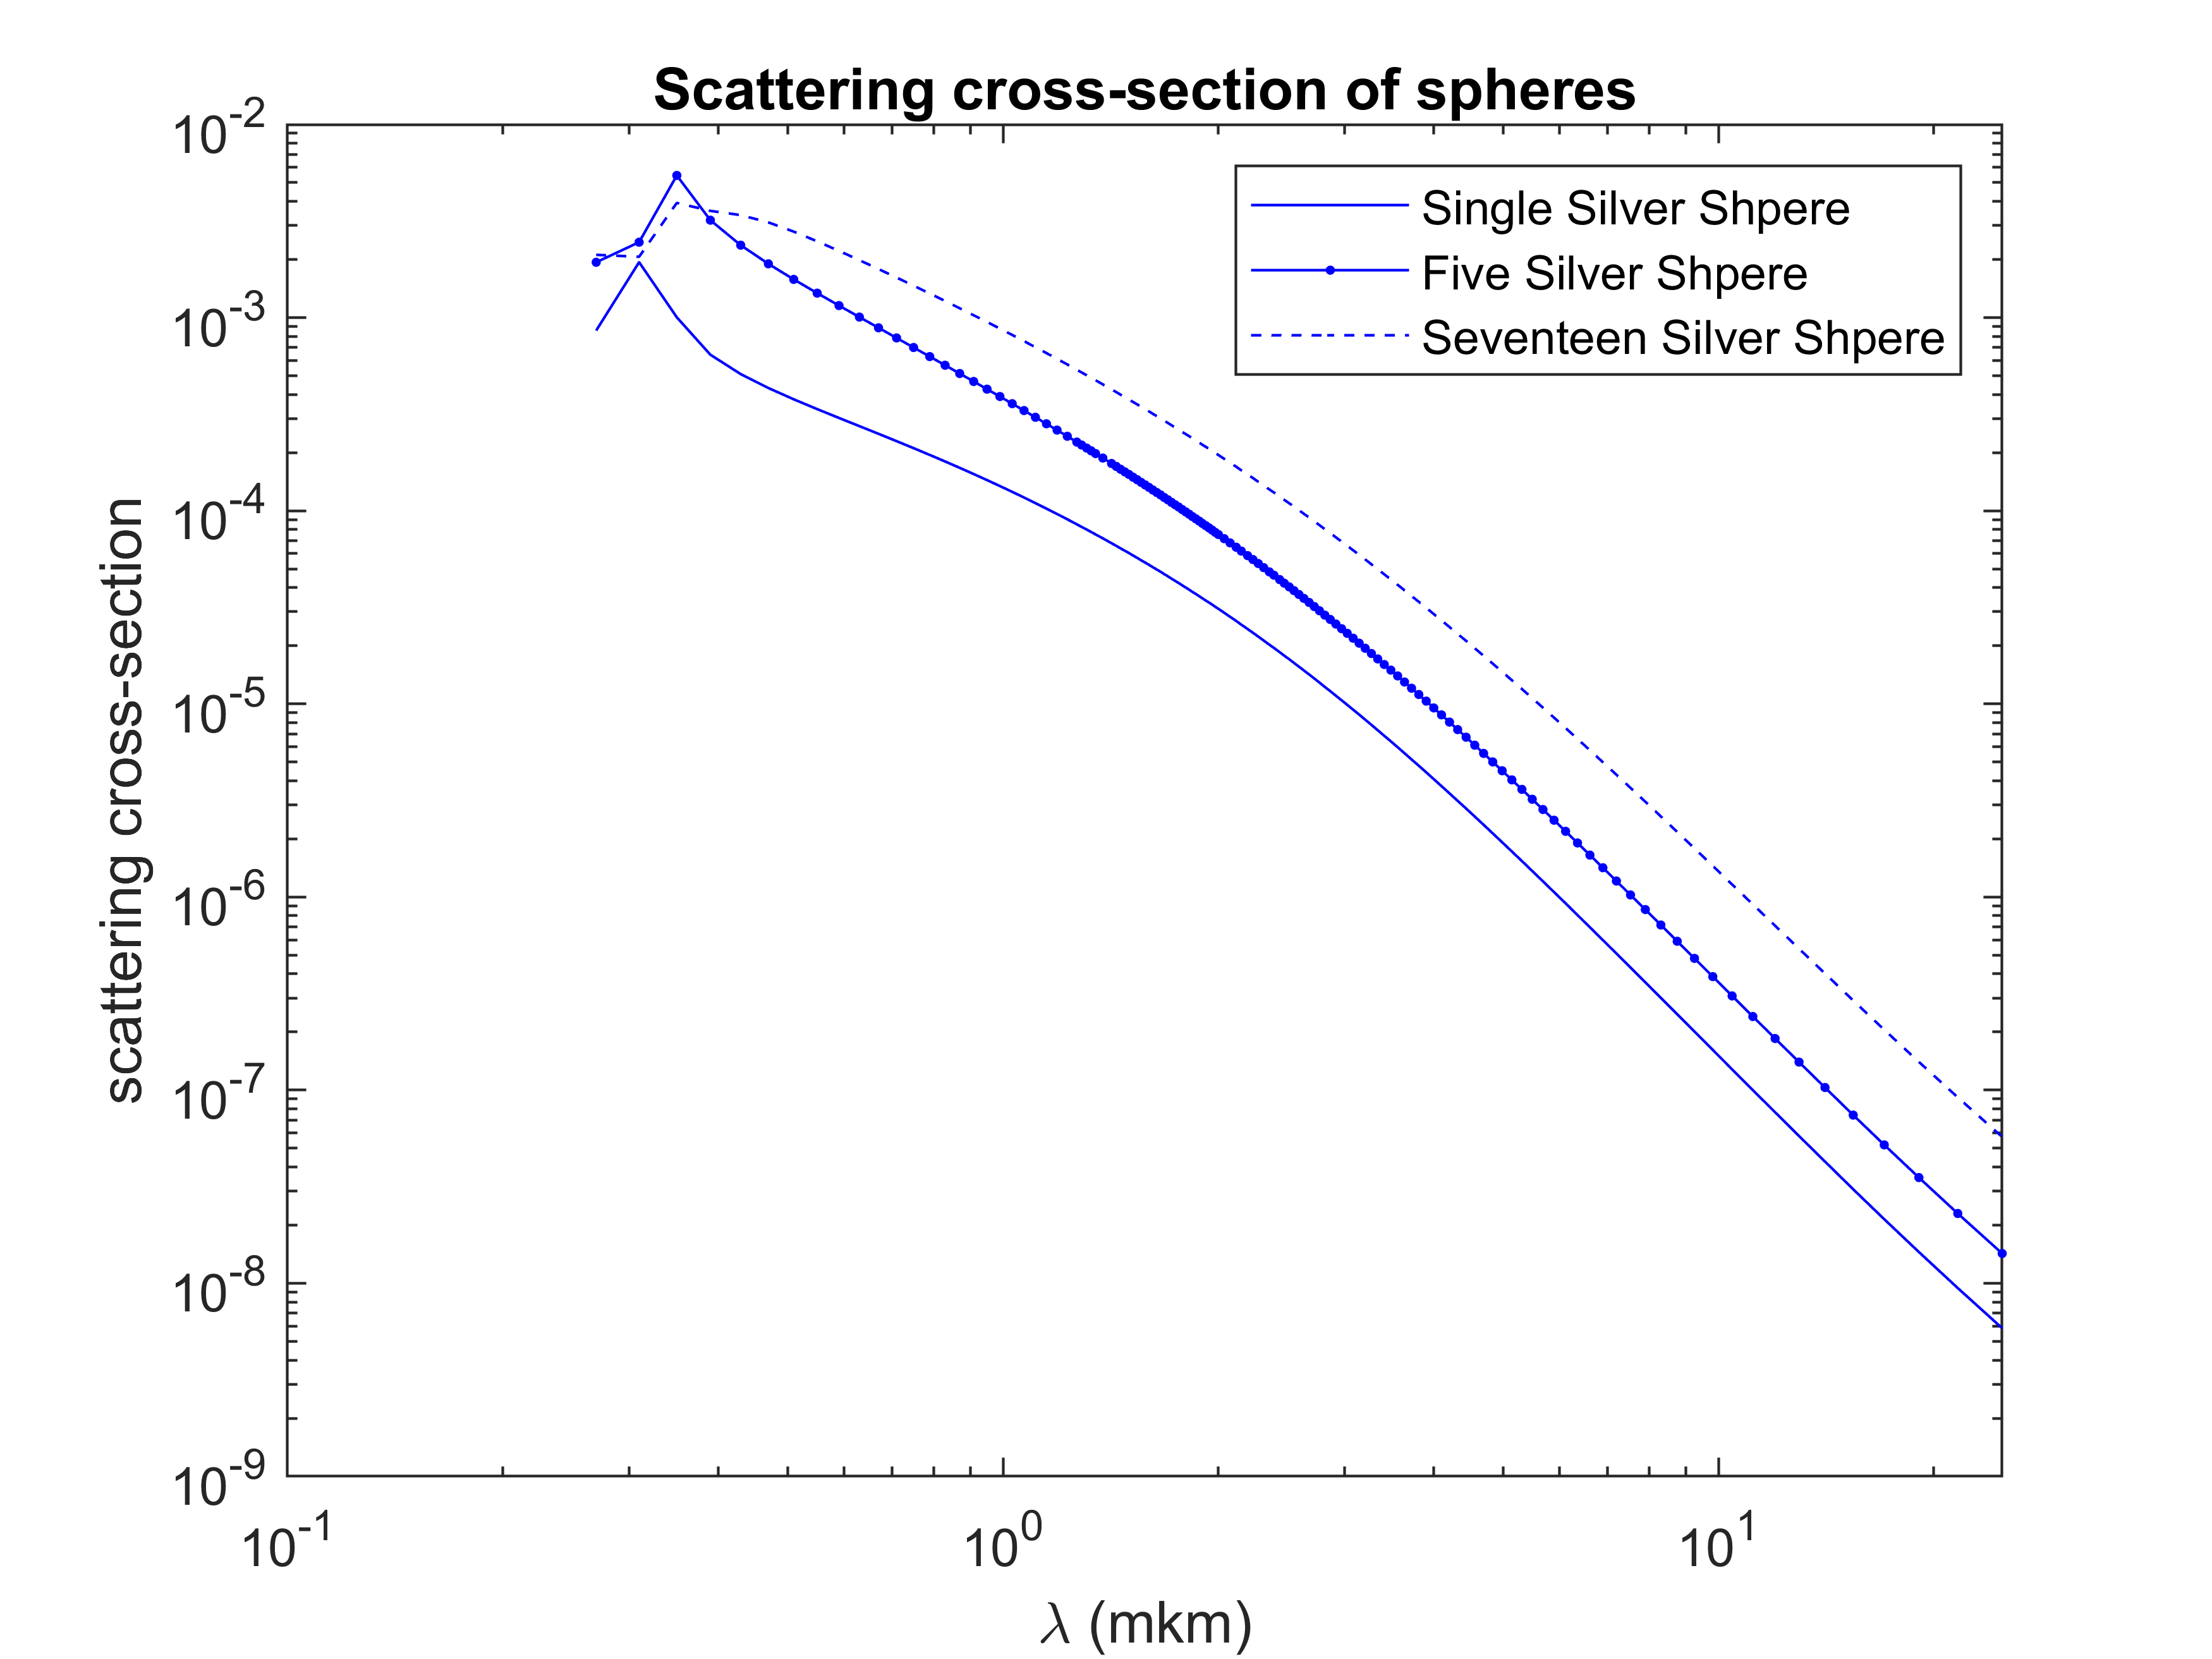
\includegraphics[width=0.8\linewidth]{scatForSilver}
	\caption{Сечение рассеяния для серебряных шаров}
	\label{fig:scatForSilver}
\end{figure} 
\begin{figure}[h!]
	\centering
	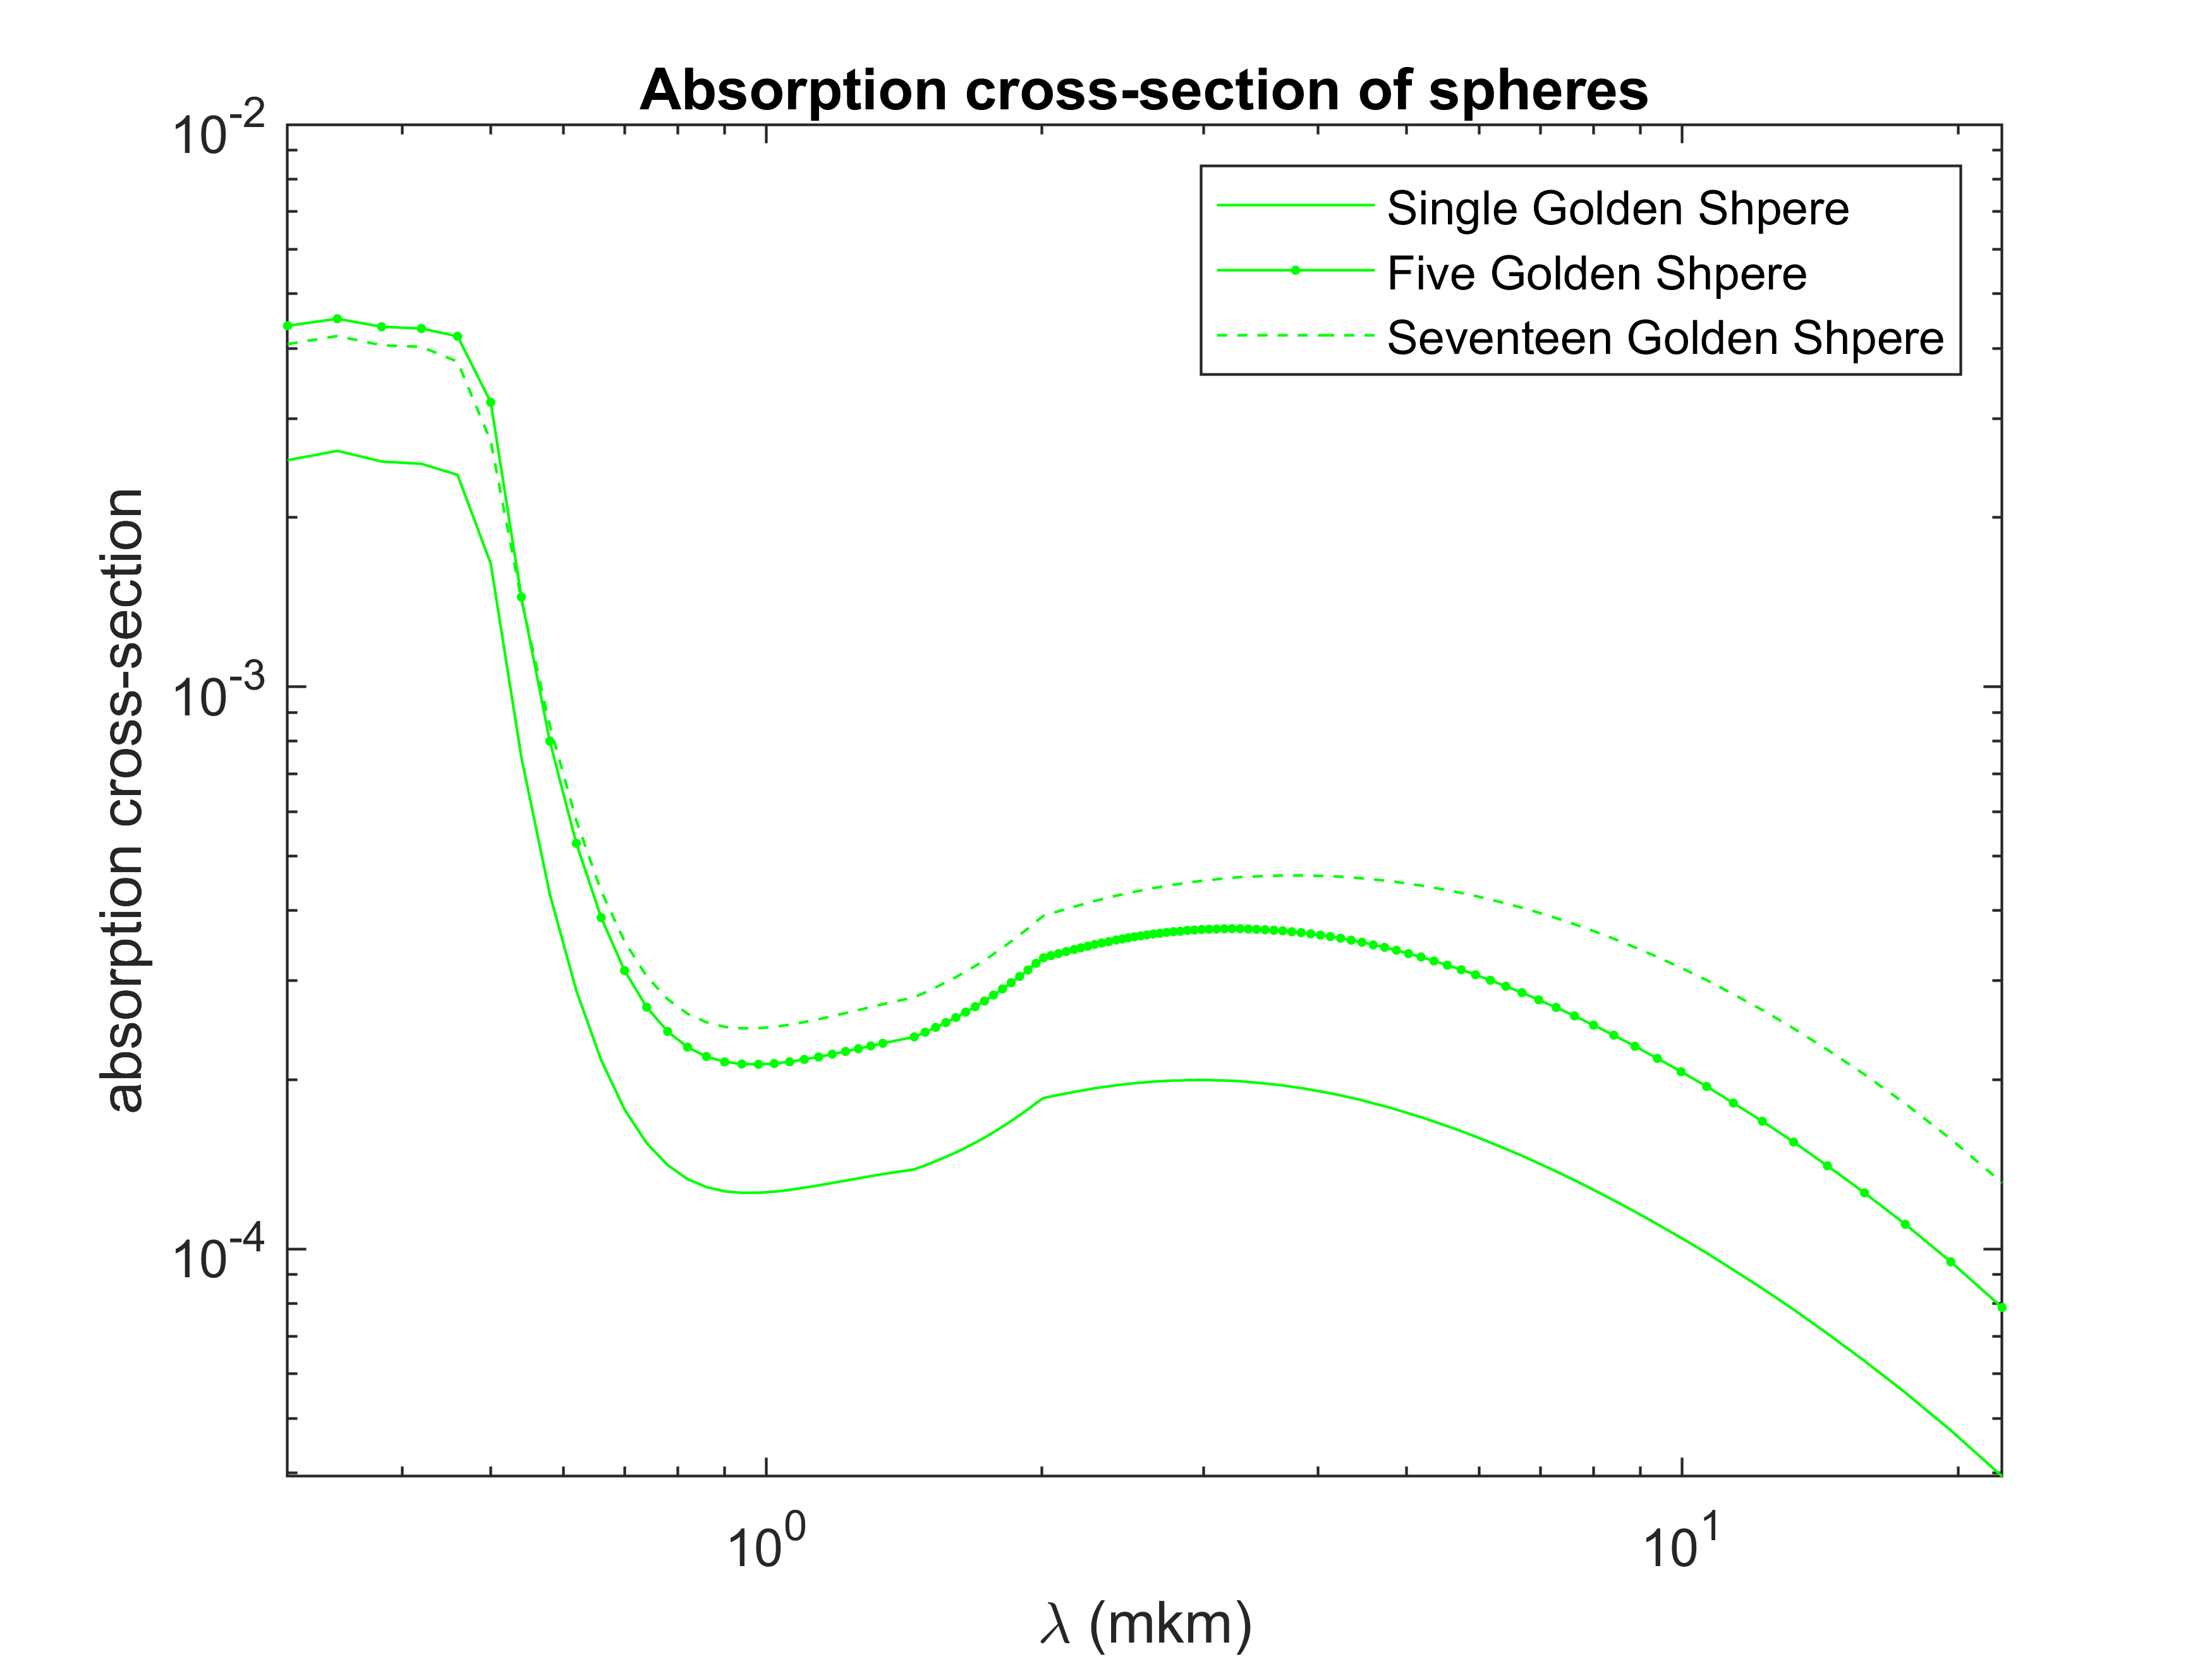
\includegraphics[width=0.8\linewidth]{absorpForGold}
	\caption{Сечение поглощения для золотых шаров}
	\label{fig:absorpForGold}
\end{figure}
\begin{figure}[h!]
	\centering
	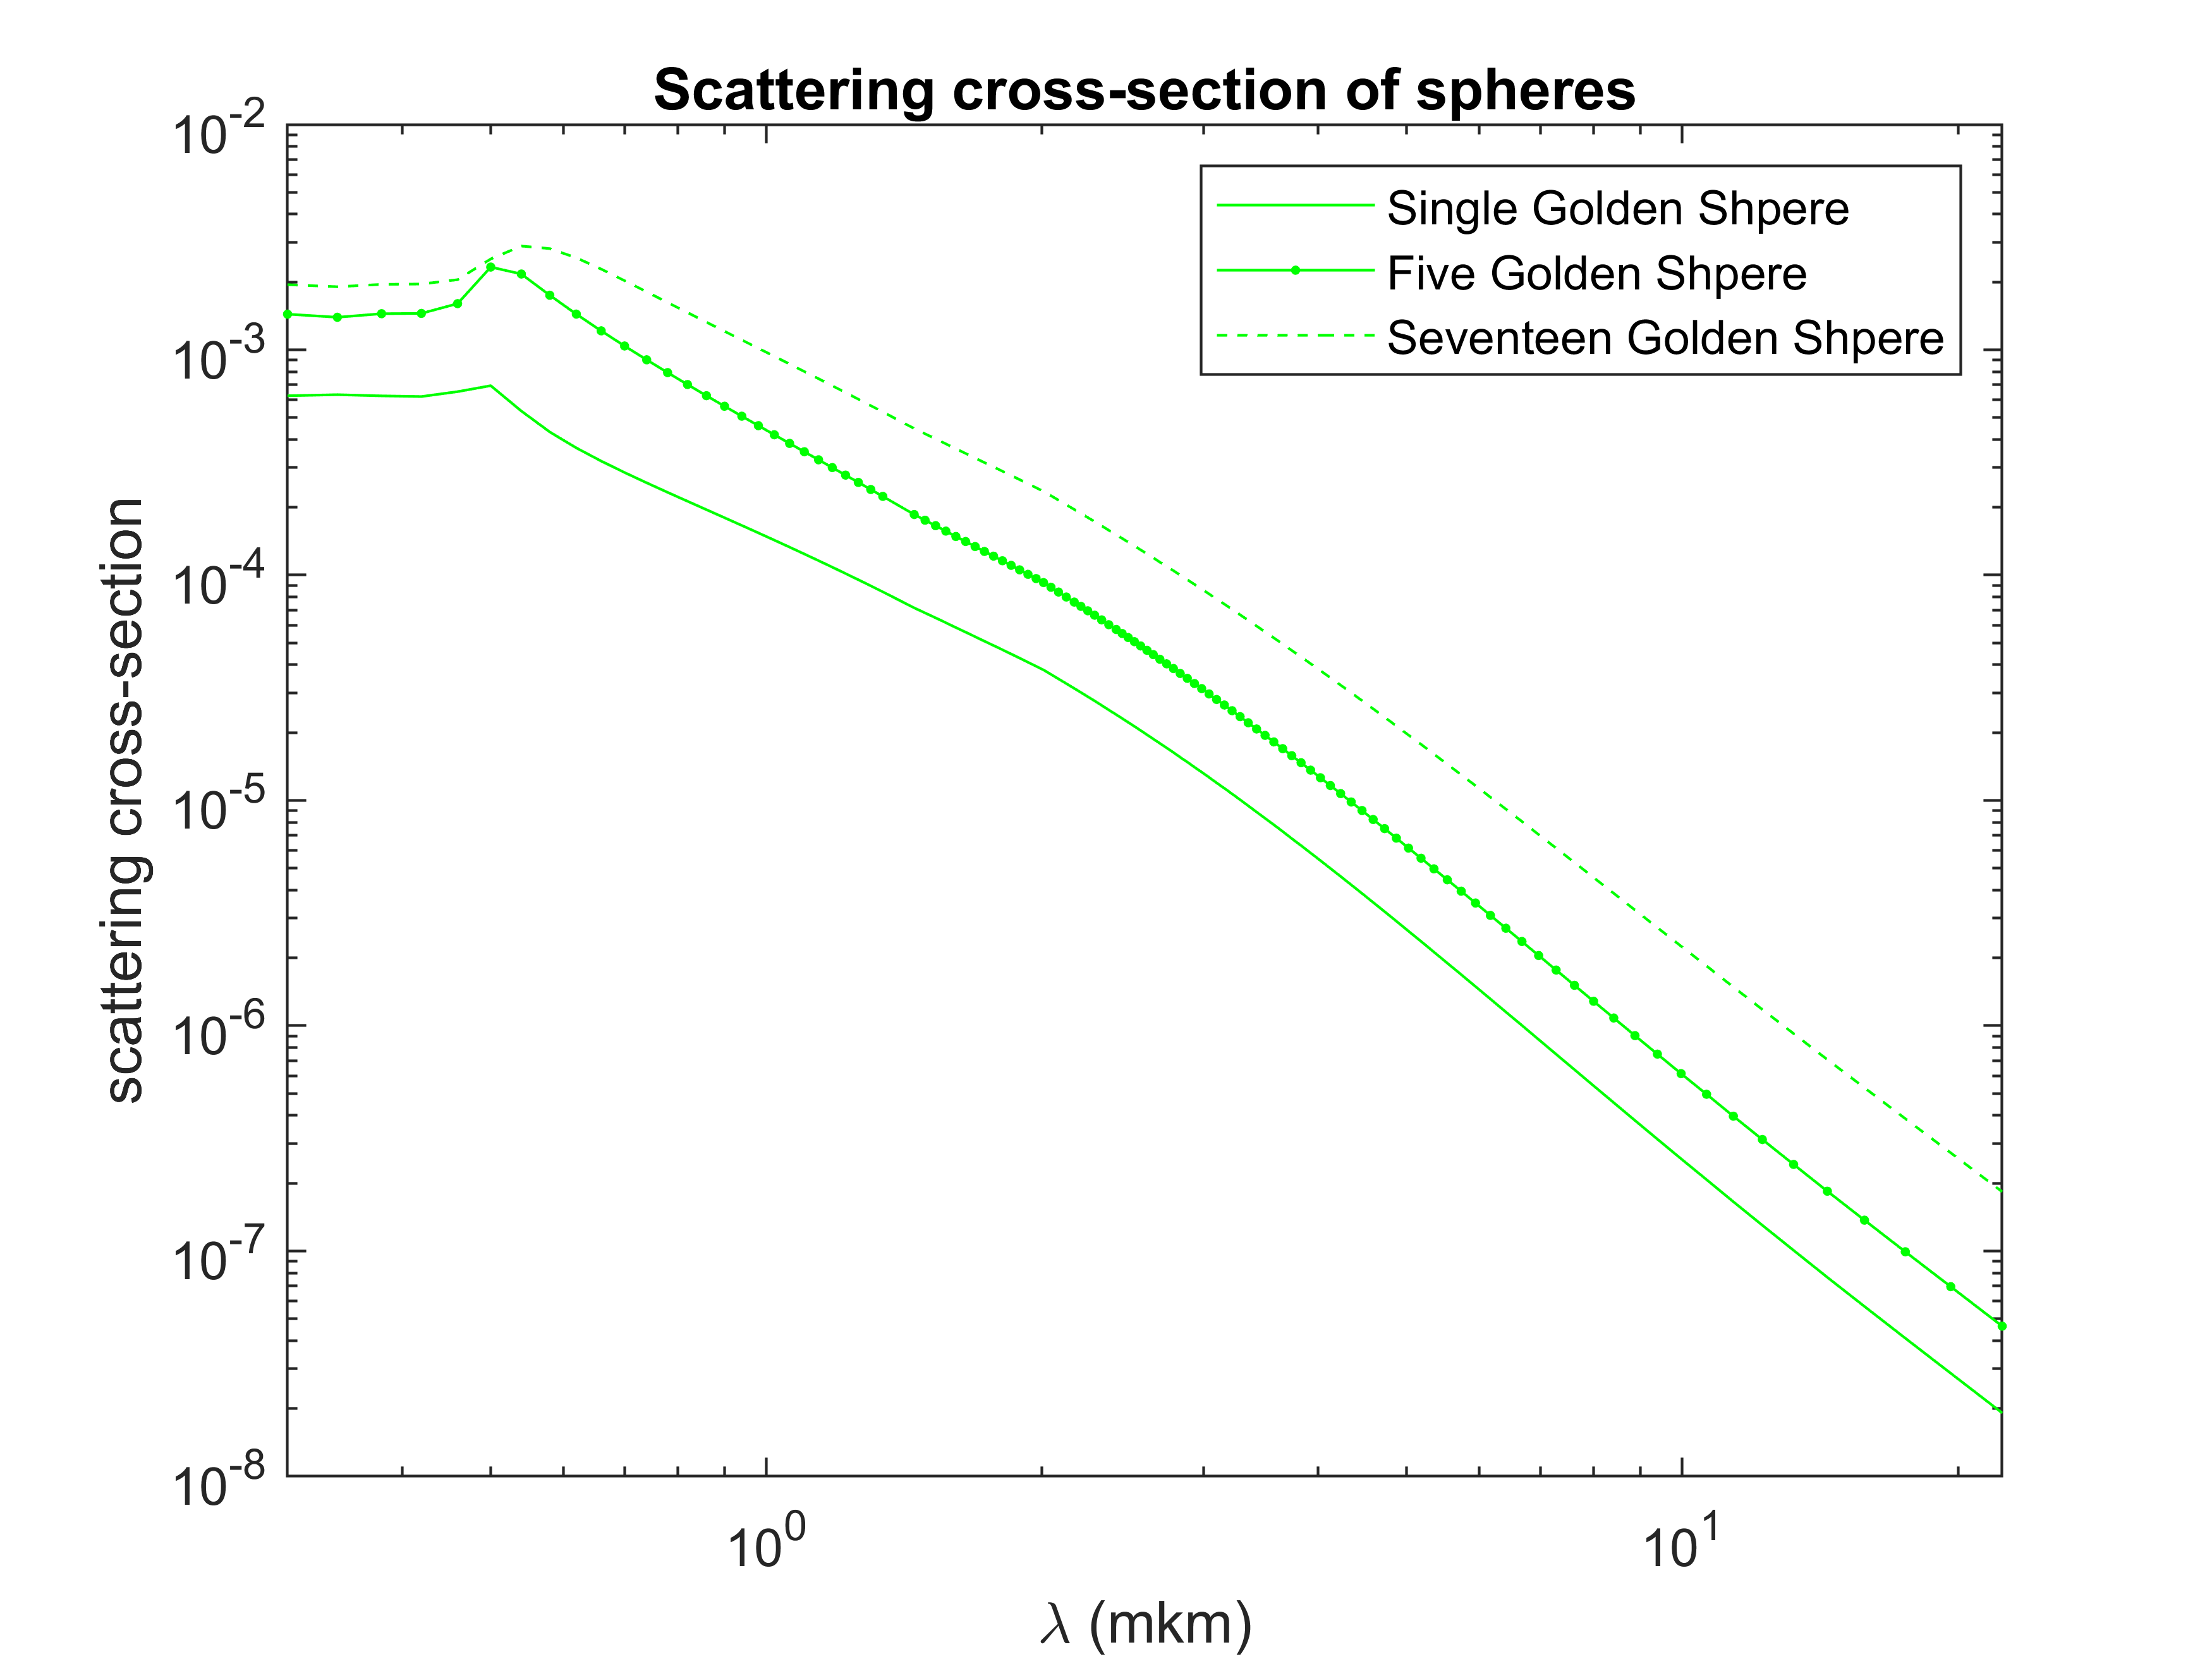
\includegraphics[width=0.8\linewidth]{scatForGold}
	\caption{Сечение рассеяния для золотых шаров}
	\label{fig:scatForGold}
\end{figure} 